\documentclass[letterpaper,12pt]{article}
\usepackage[utf8]{inputenc}
\usepackage[english]{babel}
\usepackage{graphicx}
\usepackage{amsmath}
\usepackage{amssymb}
\usepackage[margin=0.75in]{geometry}
\usepackage{chngcntr}
\usepackage{caption}
\usepackage{fancyhdr}
\usepackage{placeins}

% Adjust the header height
\setlength{\headheight}{14.5pt}
\addtolength{\topmargin}{2.5pt}
\setlength{\parskip}{1em}

% Configure section and subsection numbering
\renewcommand{\thesection}{14.\arabic{section}}
\renewcommand{\thesubsection}{14.\arabic{section}.\arabic{subsection}}

% Redefine figure counter
\captionsetup[figure]{labelformat=empty} % Avoid automatic numbering
\captionsetup[table]{labelformat=empty} % Avoid automatic numbering

% Configure fancyhdr
\pagestyle{fancy}
\fancyhf{}
\fancyhead[L]{Chapter 14}
\fancyhead[R]{\thepage}
\fancyfoot[C]{}

\title{Advanced Drive Control Schemes}
\author{}
\date{}

\begin{document}

\maketitle
\thispagestyle{fancy} % Apply fancyhdr style to the first page

\section{Introduction}

Two advanced control schemes, field-oriented control (FOC) and direct torque control (DTC), have become the industrial standards in high-power medium-voltage (MV) drives. This is in view of the following: (a) The control schemes offer superior dynamic performance; (b) their algorithms can be efficiently implemented in real time by digital processors; and (c) the cost difference between the digital implementations of advanced and low-performance control schemes is minimal.

This chapter focuses on FOC and DTC schemes for induction motor drives. It starts with an introduction to reference frame transformation, followed by dynamic models of the induction motor. Various field-oriented control schemes for the voltage and current source drives are presented. The emphasis is on the rotor flux oriented control scheme due to its simplicity and wide acceptance in the MV drives. The direct torque control is also elaborated. Important concepts are illustrated with computer simulations and experiments. The chapter ends with a comparison between the FOC and DTC schemes.

\section{Reference Frame Transformation}

The use of reference frame theory can simplify the analysis of electric machines and also provide a powerful tool for the digital implementation of sophisticated control schemes for ac drives. A number of reference frames have been proposed over the years [1], of which the stationary and synchronous reference frames are most commonly used. The transformation of variables between the two frames is presented below.

\subsection{abc/dq Frame Transformation}

The transformation of the three-phase (abc-axis) variables of an induction motor to the equivalent two-phase (dq-axis) variables can be performed by

\begin{equation}
\begin{bmatrix}
x_d \\
x_q
\end{bmatrix}
=
\frac{2}{3}
\begin{bmatrix}
\cos \theta & \cos(\theta - 2\pi/3) & \cos(\theta - 4\pi/3) \\
-\sin \theta & -\sin(\theta - 2\pi/3) & -\sin(\theta - 4\pi/3)
\end{bmatrix}
\begin{bmatrix}
x_a \\
x_b \\
x_c
\end{bmatrix} \tag{14.2-1}
\end{equation} 

where $x$ represents either current, voltage, or flux linkage, and $\theta$ is the angular displacement between the a-axis and d-axis of the three-phase and two-phase reference frames as shown in Fig. 14.2-1. The three-phase variables, $x_a, x_b$, and $x_c$, are in the \textit{stationary reference frame} which does not rotate in space whereas the two-phase variables, $x_d$ and $x_q$, are in the \textit{synchronous reference frame} whose direct (d) and quadrature (q) axes rotate in space at the synchronous speed $\omega_e$. Note that $\omega_e$ is the angular electrical (not mechanical) speed of the rotating magnetic field of the motor, given by

\begin{equation}
\omega_e = 2 \pi f_s \tag{14.2-2}
\end{equation} 

where $f_s$ is the frequency of the stator variables. The angle $\theta$ can be found from

\begin{equation}
\theta(t) = \int_{0}^{t} \omega_e(t) dt + \theta_0 \tag{14.2-3}
\end{equation} 

\begin{figure}[h]
\centering
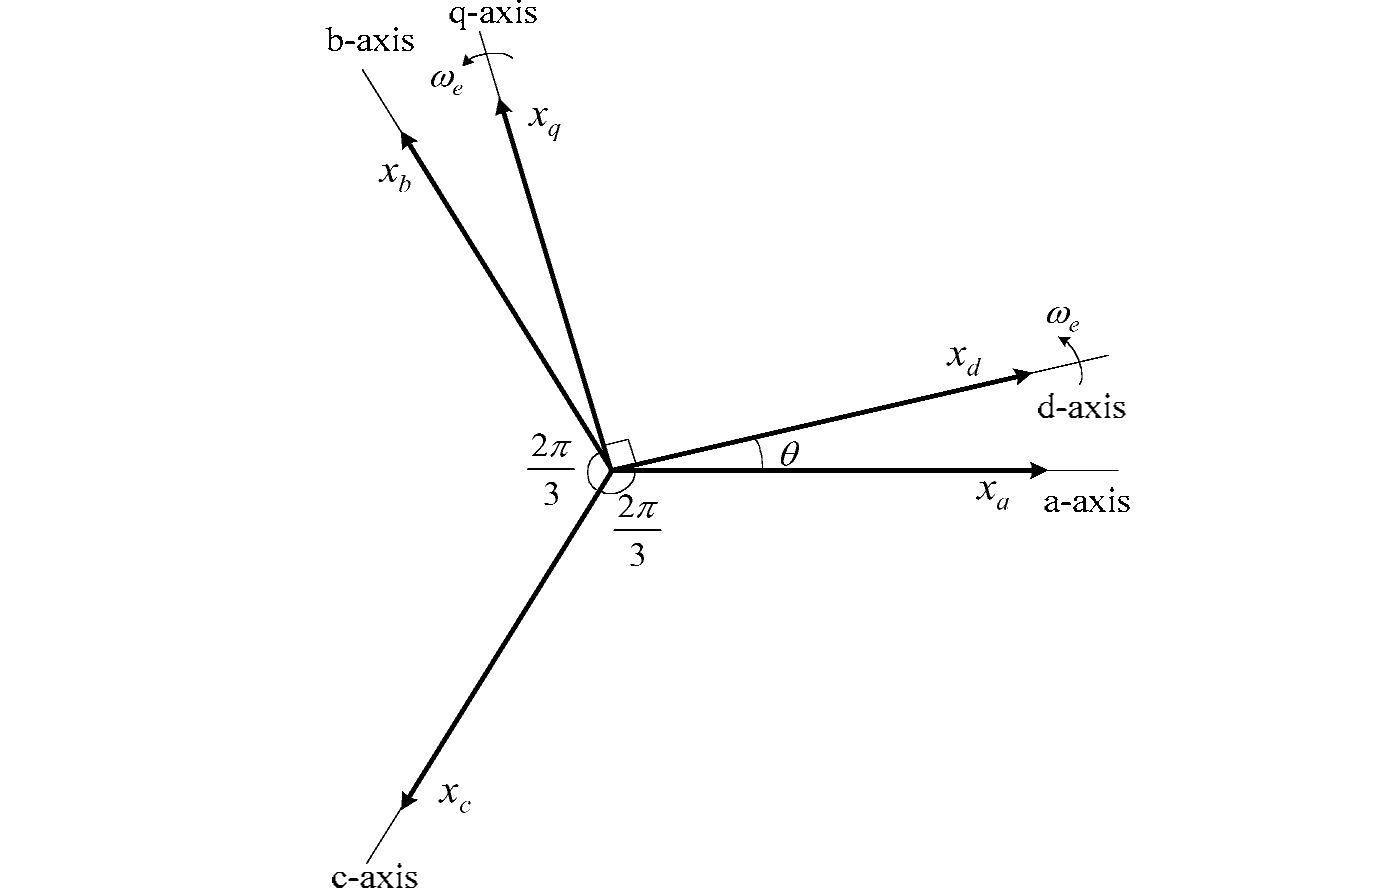
\includegraphics{graficos/img01.jpg}
\caption{Figure 14.2-1: Variables in three-phase (abc) stationary frame and two-phase (dq) synchronous frame.}
\end{figure}
\FloatBarrier

Note that the transformation equation of (14.2-1) is valid only for a three-phase balanced system, in which

\begin{equation}
x_a + x_b + x_c = 0 \tag{14.2-4}
\end{equation} 

Similarly, the two-phase variables in the synchronous frame can be transformed back to the three-phase stationary frame by

\begin{equation}
\begin{bmatrix}
x_a \\
x_b \\
x_c
\end{bmatrix}
=
\begin{bmatrix}
\cos \theta & -\sin \theta \\
\cos(\theta - 2\pi/3) & -\sin(\theta - 2\pi/3) \\
\cos(\theta - 4\pi/3) & -\sin(\theta - 4\pi/3)
\end{bmatrix}
\begin{bmatrix}
x_d \\
x_q
\end{bmatrix} \tag{14.2-5}
\end{equation} 

which is referred to as dq/abc transformation.

The relationship between a space vector and its phase variables is illustrated in Fig. 14.2-2a, where a current space vector $\vec{i}_s$ rotates at a certain speed $\omega$ in the stationary frame (refer to Chapter 6 for space vector definition). Its phase currents $i_{as}, i_{bs}$, and $i_{cs}$ can be obtained by decomposing $\vec{i}_s$ onto their corresponding abc-axes. Since the three axes are stationary in space, each of the phase currents varies one cycle over time when $\vec{i}_s$ rotates one revolution in space. If the length (magnitude) and the rotating speed of $\vec{i}_s$ are constant, the waveforms of the phase currents over time are sinusoidal with a phase displacement of $2\pi/3$ between each other.

\begin{figure}[h]
\centering
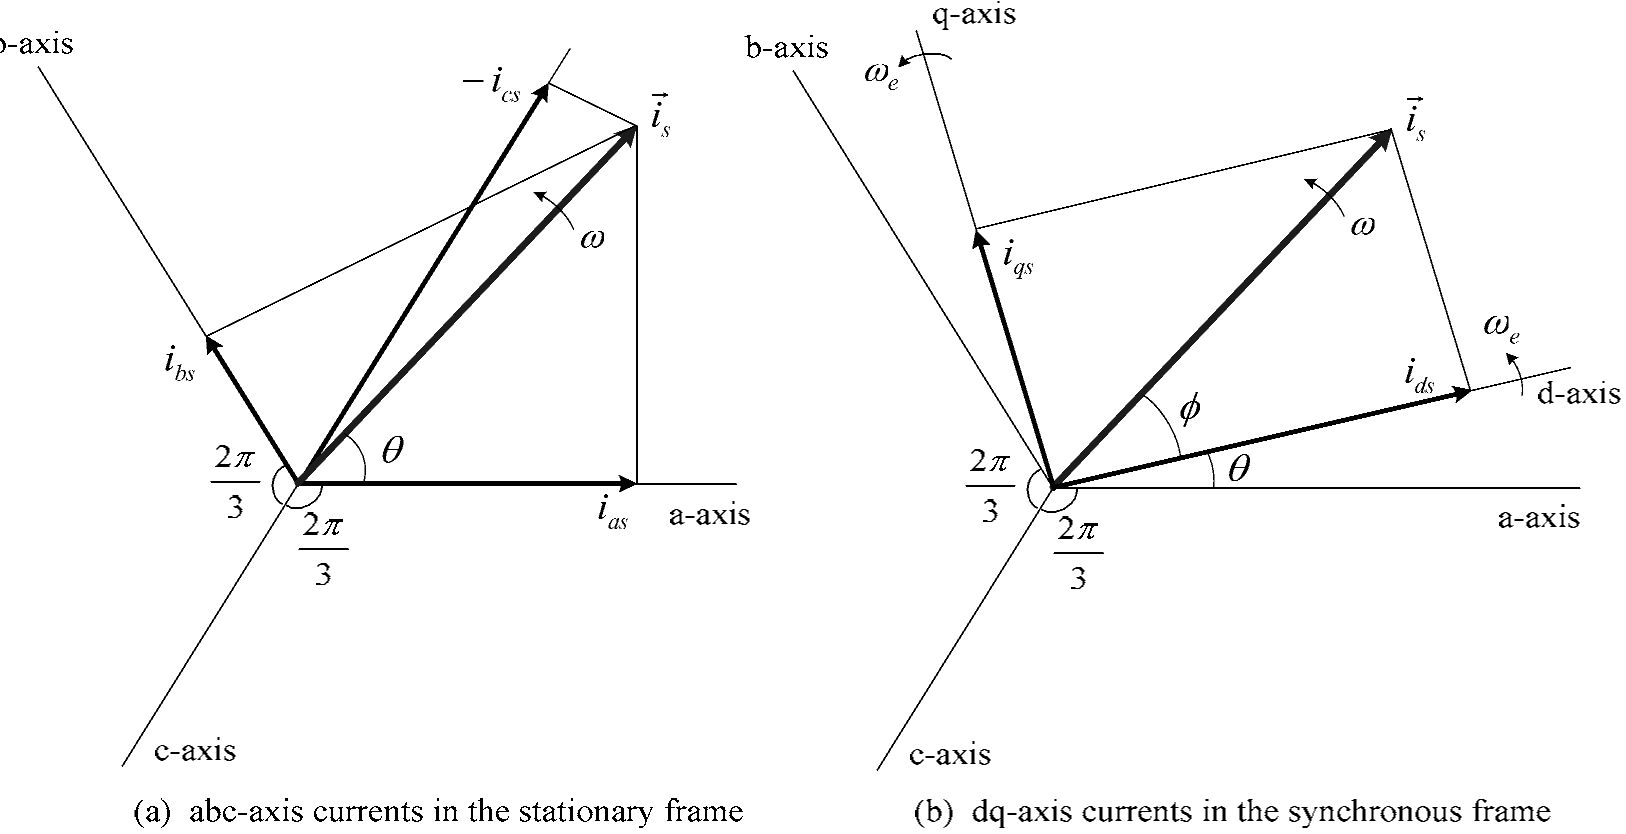
\includegraphics{graficos/img02.jpg}
\caption{Figure 14.2-2: Decomposition of current vector $\vec{i}_s$.}
\end{figure}
\FloatBarrier

Figure 14.2-2b illustrates another case where the current vector $\vec{i}_s$ is in the dq-axis synchronous reference frame. Assuming that $\vec{i}_s$ rotates at the same speed as that of the dq-axis frame, the stator current angle $\phi$, which is the angle between $\vec{i}_s$ and the d-axis, is constant. The resultant dq-axis current components, $i_{ds}$ and $i_{qs}$, are of dc signals. As will be seen in the subsequent sections, this transformation can be utilized to simplify the simulation, design, and digital implementation of drive systems, where a three-phase ac signal can be effectively represented by a two-phase dc signal.

\subsection{3/2 Stationary Transformation}

With the rotating speed of the two-phase reference frame set at zero and its d-axis coincident with the a-axis of the three-phase frame ($\omega_e = 0$ and $\theta = 0$), both frames are stationary in space. The transformation of the three-phase variables to the two-phase variables can be obtained by setting $\theta$ in (14.2-1) to zero, from which

\begin{equation}
\begin{bmatrix}
x_d \\
x_q
\end{bmatrix}
=
\frac{2}{3}
\begin{bmatrix}
1 & -1/2 & -1/2 \\
0 & \sqrt{3}/2 & -\sqrt{3}/2
\end{bmatrix}
\begin{bmatrix}
x_a \\
x_b \\
x_c
\end{bmatrix} \tag{14.2-6}
\end{equation}

The above transformation is referred to as 3/2 transformation in this book. It is worth noting that the d-axis variable can be expressed as

\begin{equation}
x_d = \frac{2}{3} \left( x_a - \frac{1}{2}x_b - \frac{1}{2}x_c \right) = x_a \tag{14.2-7}
\end{equation}

which is equal to the a-axis variable $x_a$.

Similarly, the two-phase to three-phase stationary transformation, which is denoted 2/3 transformation, can be performed by

\begin{equation}
\begin{bmatrix}
x_a \\
x_b \\
x_c
\end{bmatrix}
=
\begin{bmatrix}
1 & 0 \\
-1/2 & \sqrt{3}/2 \\
-1/2 & -\sqrt{3}/2
\end{bmatrix}
\begin{bmatrix}
x_d \\
x_q
\end{bmatrix} \tag{14.2-8}
\end{equation}

\section{Induction Motor Dynamic Models}

There are two commonly used dynamic models for the induction motor. One is based on space vector theory and the other is derived from dq-axis theory. The space vector model features compact mathematical expressions and concise space vector diagram, whereas the dq-axis model does not need to use complex numbers or variables. Both models are equally valid for the analysis of transient and steady-state performance of the induction motor. In what follows, the two models are presented and their relationship is revealed.

\subsection{Space Vector Motor Model}

It is assumed in the following analysis that the induction motor is three-phase symmetrical and its magnetic core is linear with a negligible core loss. The space vector model for an induction motor is generally composed of three sets of equations [2]. The first set is the voltage equations, given by

\begin{equation}
\vec{v}_s = R_s \vec{i}_s + p \vec{\lambda}_s + j\omega \vec{\lambda}_s \tag{14.3-1}
\end{equation}

\begin{equation}
\vec{v}_r = R_r \vec{i}_r + p \vec{\lambda}_r + j(\omega - \omega_r)\vec{\lambda}_r \tag{14.3-1}
\end{equation}

where $\vec{v}_s$ and $\vec{v}_r$ are the stator and rotor voltage vectors, respectively; $\vec{i}_s$ and $\vec{i}_r$ are the stator and rotor current vectors, respectively; $\vec{\lambda}_s$ and $\vec{\lambda}_r$ are the stator and rotor flux-linkage vectors, respectively; $R_s$, $R_r$ are the stator and rotor winding resistance, respectively; $\omega$ is the rotating speed of an arbitrary reference frame; $\omega_r$ is the rotor angular speed (electrical); and $p$ is the derivative operator ($p = d/dt$).

The terms $j\omega \vec{\lambda}_s$ and $j(\omega - \omega_r)\vec{\lambda}_r$ on the right-hand side of (14.3-1) are referred to as speed voltages, which are induced by the rotation of the reference frame.

The second set is the flux-linkage equations

\begin{equation}
\vec{\lambda}_s = L_s \vec{i}_s + L_m \vec{i}_r \tag{14.3-2}
\end{equation}

\begin{equation}
\vec{\lambda}_r = L_r \vec{i}_r + L_m \vec{i}_s \tag{14.3-2}
\end{equation}

where $L_s = L_{ls} + L_m$ represents the stator self-inductance; $L_r = L_{lr} + L_m$ represents the rotor self-inductance; $L_{ls}$ and $L_{lr}$ are the stator and rotor leakage inductances, respectively; and $L_m$ is the magnetizing inductance. Note that all the rotor parameters and variables, such as $R_r$, $L_{lr}$, $\vec{i}_r$, and $\vec{\lambda}_r$, in the above equations are referred to the stator side.

The third set is the motion equation, given by

\begin{equation}
\frac{J}{P} p\omega_r = T_e - T_L \tag{14.3-3}
\end{equation}

\begin{equation}
T_e = \frac{3P}{2} \text{Re}(\vec{J} \vec{\lambda}_s \vec{i}_s^*) = -\frac{3P}{2} \text{Re}(\vec{J} \vec{\lambda}_r \vec{i}_r^*) \tag{14.3-3}
\end{equation}

where $J$ is the total moment of inertia of the rotor and load, $P$ is the number of pole pairs, $T_L$ is the load torque, and $T_e$ is the electromagnetic torque.

The above equations constitute the space vector model of the induction motor whose schematic representation is given in Fig. 14.3-1. The motor model is in the arbitrary reference frame that rotates in space at the arbitrary speed of $\omega$.

\begin{figure}[h]
\centering
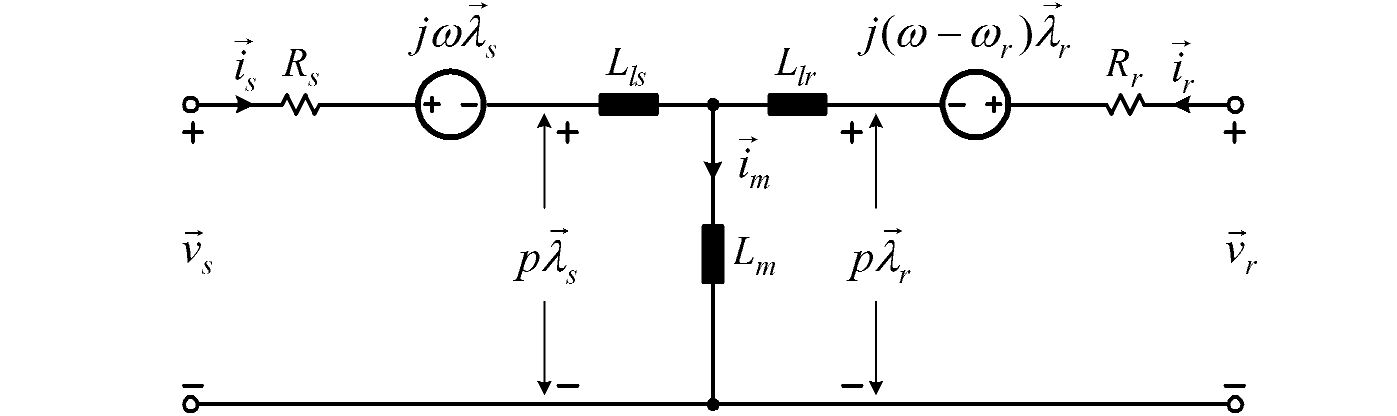
\includegraphics{graficos/img03.jpg}
\caption{Figure 14.3-1: Space vector model of an induction motor in the arbitrary reference frame.}
\end{figure}
\FloatBarrier

In the simulation and digital implementation of advanced control systems, the motor models in the synchronous and stationary reference frames are often employed. The synchronous-frame motor model can be easily obtained by setting the arbitrary speed $\omega$ in (14.3-1) to the synchronous speed $\omega_e$. Figure 14.3-2a shows the equivalent circuit of a squirrel cage motor in the synchronous frame, where the rotor winding is shorted ($\vec{v}_r = 0$) and $\omega_{sl}$ is the angular slip frequency, given by

\begin{equation}
\omega_{sl} = \omega_e - \omega_r \tag{14.3-4}
\end{equation}

To obtain the model in the stationary (stator) frame, we can set the arbitrary speed $\omega$ of the rotating reference frame to zero. The resultant equivalent circuit is shown in Fig. 14.3-2b.

\begin{figure}[h]
\centering
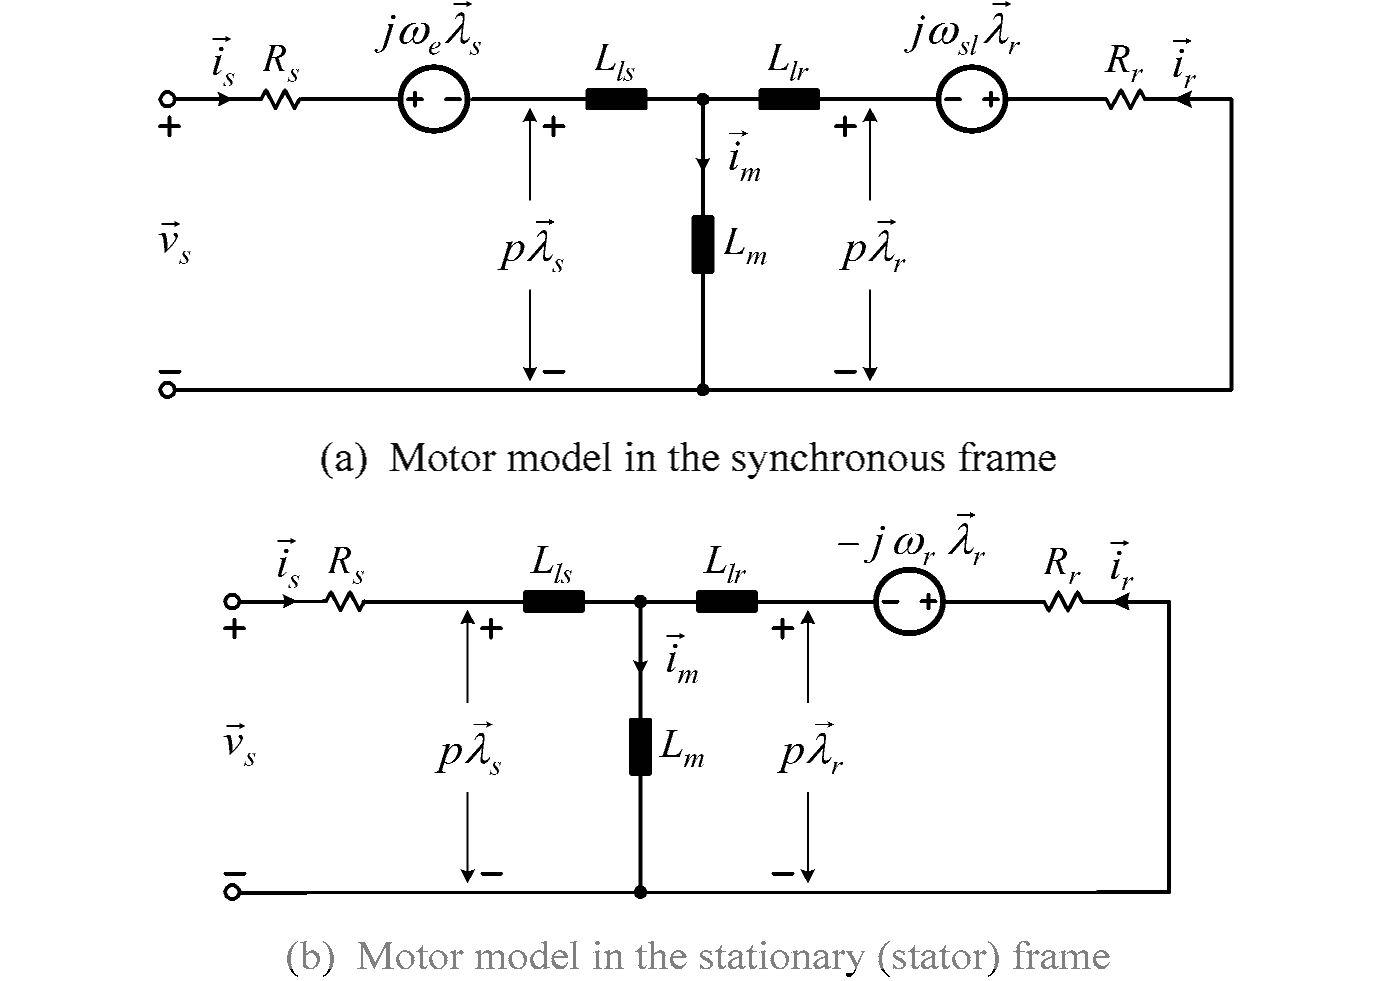
\includegraphics{graficos/img04.jpg}
\caption{Figure 14.3-2: Space vector models for a squirrel cage induction motor.}
\end{figure}
\FloatBarrier

\subsection{dq-Axis Motor Model}

The induction motor dq-axis model can be derived using three-phase circuit theory and then transformed into the two-phase (dq-axis) frame [1]. Alternatively, it can

also be obtained by decomposing the space vectors in the space vector motor model into the d- and q-axis components [2], that is,

\begin{equation}
\vec{v}_s = v_{ds} + jv_{qs}, \quad \vec{i}_s = i_{ds} + ji_{qs}, \quad \vec{\lambda}_s = \lambda_{ds} + j\lambda_{qs} \tag{14.3-5}
\end{equation}

\begin{equation}
\vec{v}_r = v_{dr} + jv_{qr}, \quad \vec{i}_r = i_{dr} + ji_{qr}, \quad \vec{\lambda}_r = \lambda_{dr} + j\lambda_{qr} \tag{14.3-5}
\end{equation}

Substituting (14.3-5) to (14.3-1), the dq-axis voltage equations for the induction motor can be obtained:

\begin{equation}
v_{ds} = R_s i_{ds} + p\lambda_{ds} - \omega \lambda_{qs} \tag{14.3-6}
\end{equation}
\begin{equation}
v_{qs} = R_s i_{qs} + p\lambda_{qs} + \omega \lambda_{ds} \tag{14.3-6}
\end{equation}
\begin{equation}
v_{dr} = R_r i_{dr} + p\lambda_{dr} - (\omega - \omega_r)\lambda_{dr} \tag{14.3-6}
\end{equation}
\begin{equation}
v_{qr} = R_r i_{qr} + p\lambda_{qr} + (\omega - \omega_r)\lambda_{dr} \tag{14.3-6}
\end{equation}

where the stator and rotor flux-linkages can be calculated by

\begin{equation}
\lambda_{ds} = L_s i_{ds} + L_m (i_{ds} + i_{dr}) \tag{14.3-7}
\end{equation}
\begin{equation}
\lambda_{qs} = L_s i_{qs} + L_m (i_{qs} + i_{qr}) \tag{14.3-7}
\end{equation}
\begin{equation}
\lambda_{dr} = L_r i_{dr} + L_m (i_{ds} + i_{dr}) \tag{14.3-7}
\end{equation}
\begin{equation}
\lambda_{qr} = L_r i_{qr} + L_m (i_{qs} + i_{qr}) \tag{14.3-7}
\end{equation}

The electromagnetic torque can be expressed in a number of ways. Some of the commonly used expressions are

\begin{equation}
T_e = \left\{
\begin{array}{l}
\frac{3P}{2}(i_{qs}\lambda_{ds} - i_{ds}\lambda_{qs}) \\
\frac{3PL_m}{2}(i_{qs}i_{dr} - i_{ds}i_{qr}) \\
\frac{3PL_m}{2L_r}(i_{qs}\lambda_{dr} - i_{ds}\lambda_{qr})
\end{array} \tag{14.3-8}
\right.
\end{equation}

Equations (14.3-6) to (14.3-8) together with the motion equation of (14.3-3) represent the dq-axis model of the induction motor, whose equivalent circuit is shown in Fig. 14.3-3.

\begin{figure}[h]
\centering
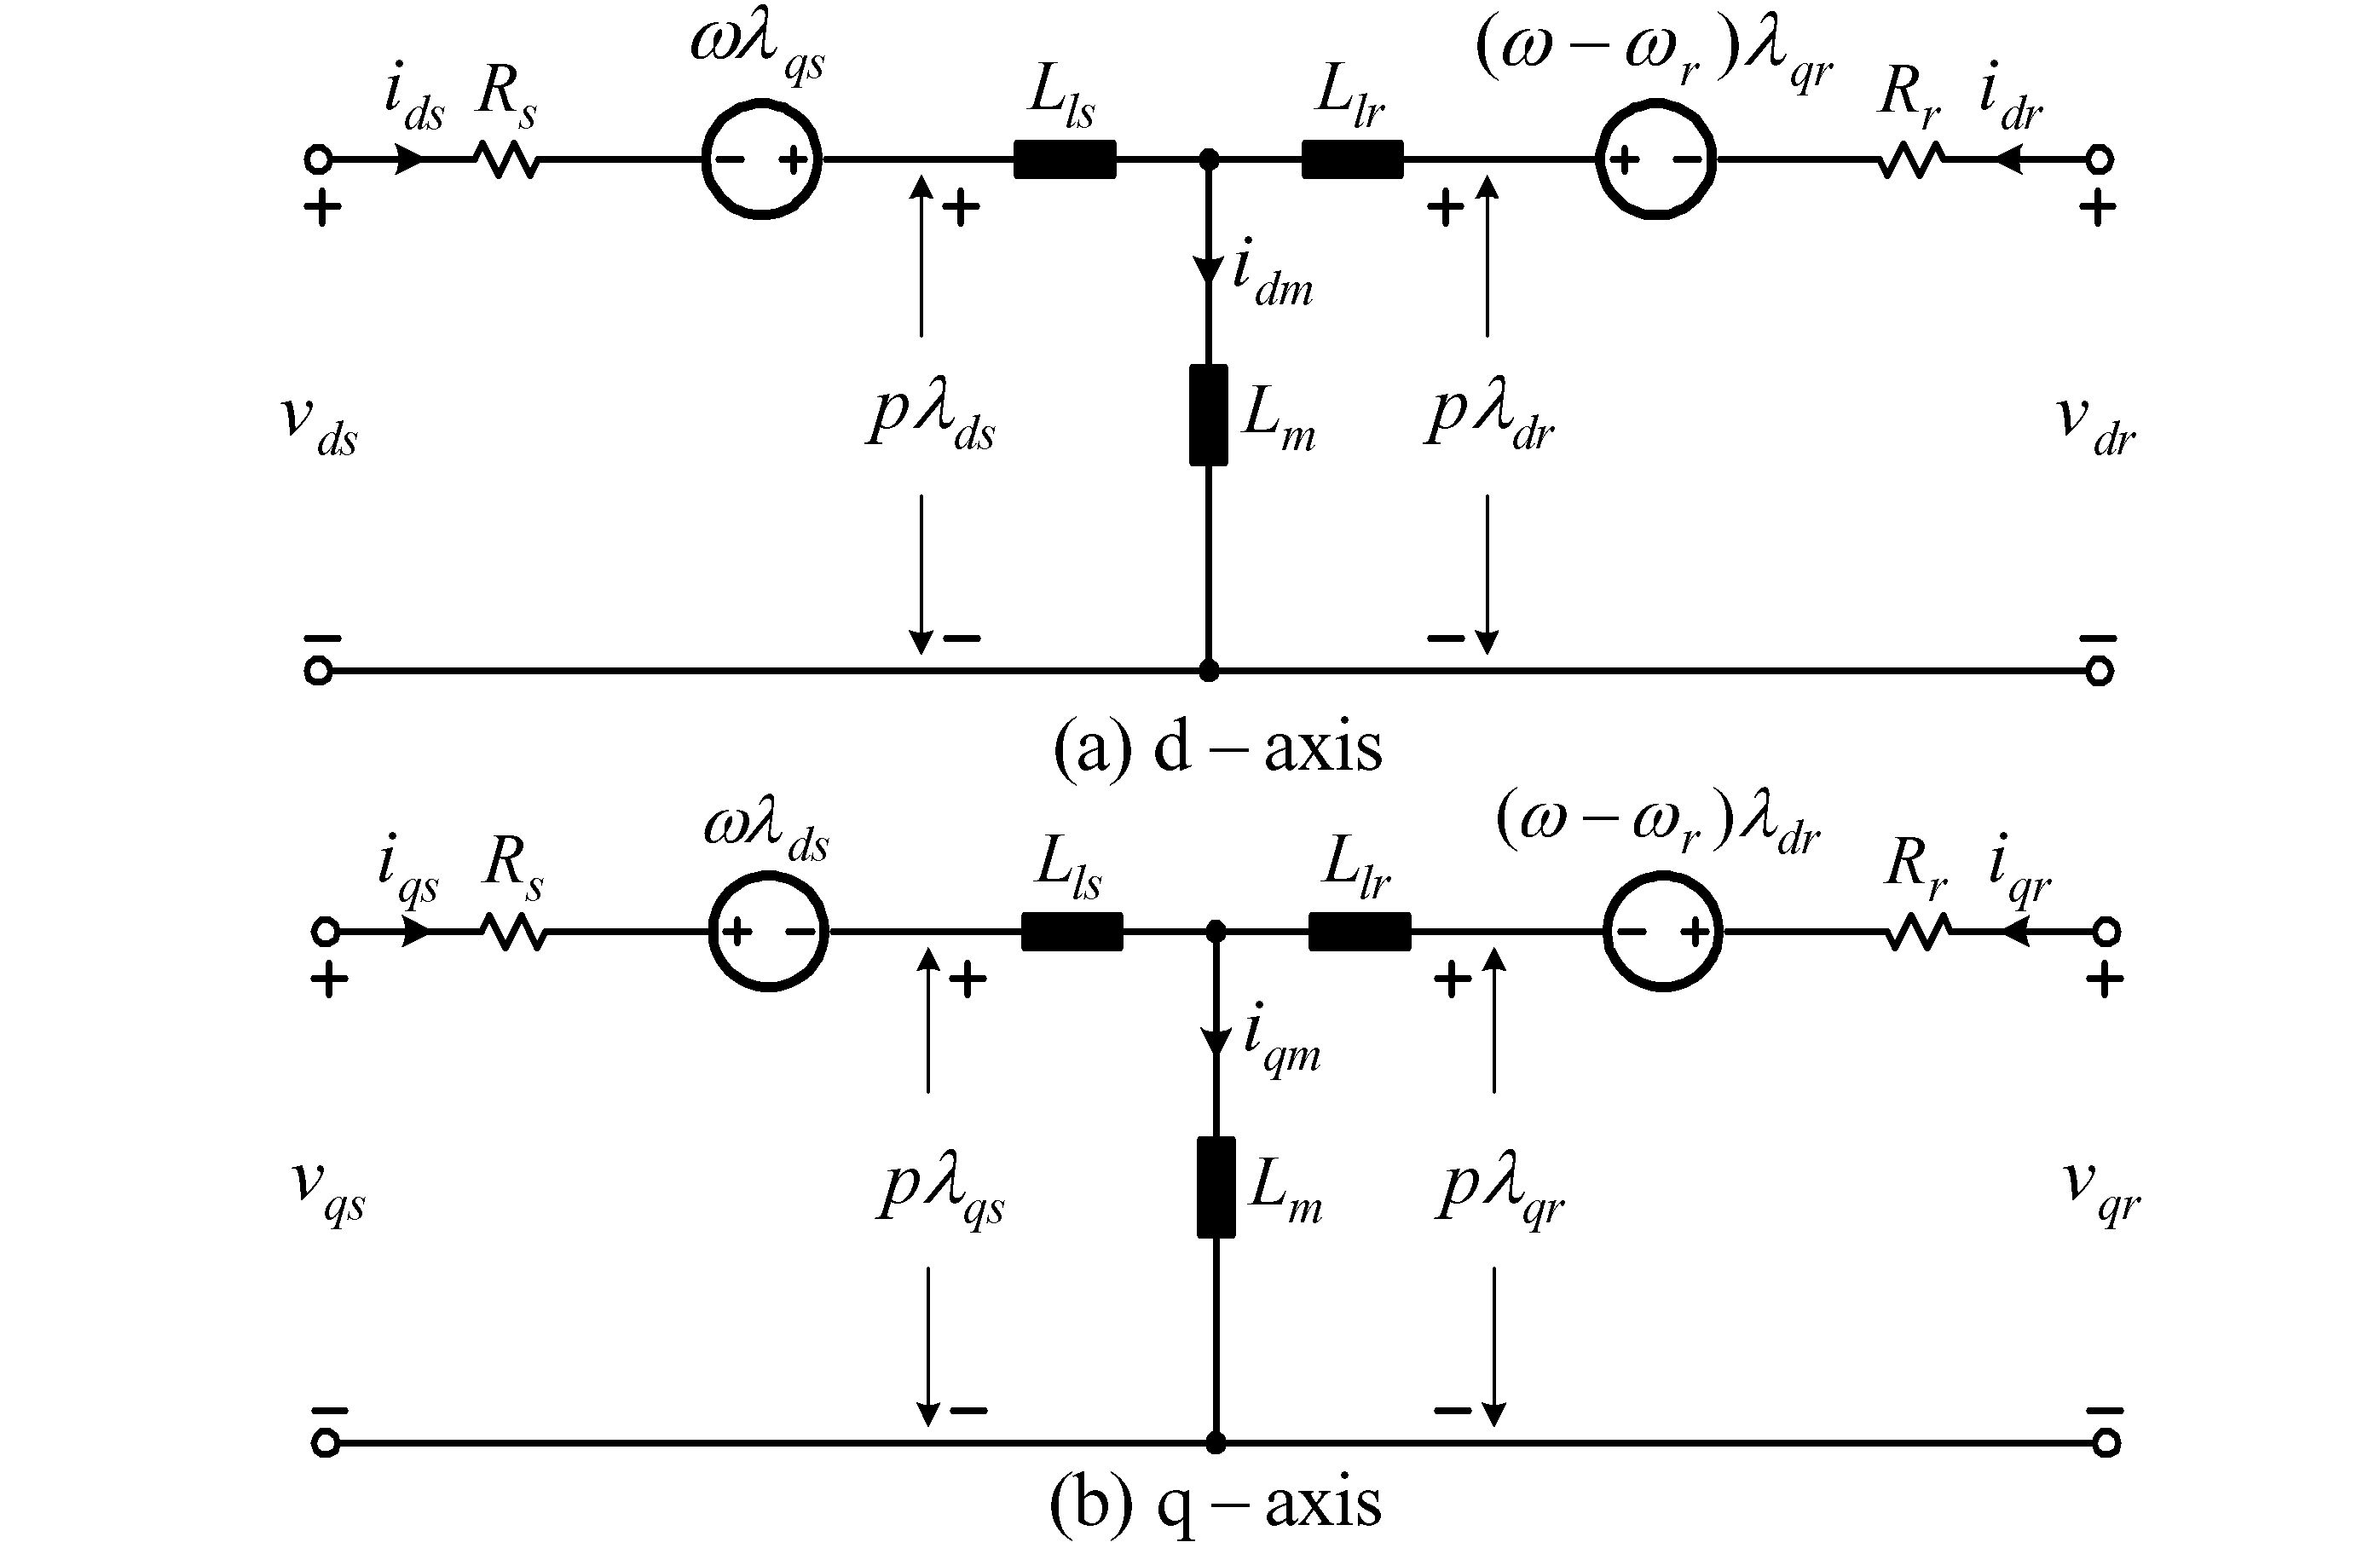
\includegraphics{graficos/img05.jpg}
\caption{Figure 14.3-3: Induction motor dq-axis model in the arbitrary reference frame.}
\end{figure}
\FloatBarrier

\subsection{Induction Motor Transient Characteristics}

It is instructive to study transient characteristics of the induction motor during free acceleration using the dynamic motor models. The motor under investigation is a low-power squirrel cage motor with the following parameters: $V_{LL} = 208 \, V$, 60Hz, $Z_{base} = 15.4 \, \Omega$, $R_s = 0.068 \, pu$, $R_r = 0.045 \, pu$, $L_{ls} = L_{lr} = 0.058 \, pu$, $L_m = 1.95 \, pu$, $P = 1$, and $J = 0.02 \, kg\cdot m^2$. Figure 14.3-4 shows the block diagram for computer simulation with the motor model in the stationary frame ($\omega = 0$). The three-phase supply voltages $v_{as}$, $v_{bs}$, and $v_{cs}$ are transformed to the dq-axis stator voltages $v_{ds}$ and $v_{qs}$ by the 3/2 transformation. The simulated dq-axis stator currents $i_{ds}$ and $i_{qs}$ are then converted to the three-phase currents $i_{as}$, $i_{bs}$, and $i_{cs}$ by the 2/3 transformation.

\begin{figure}[h]
\centering
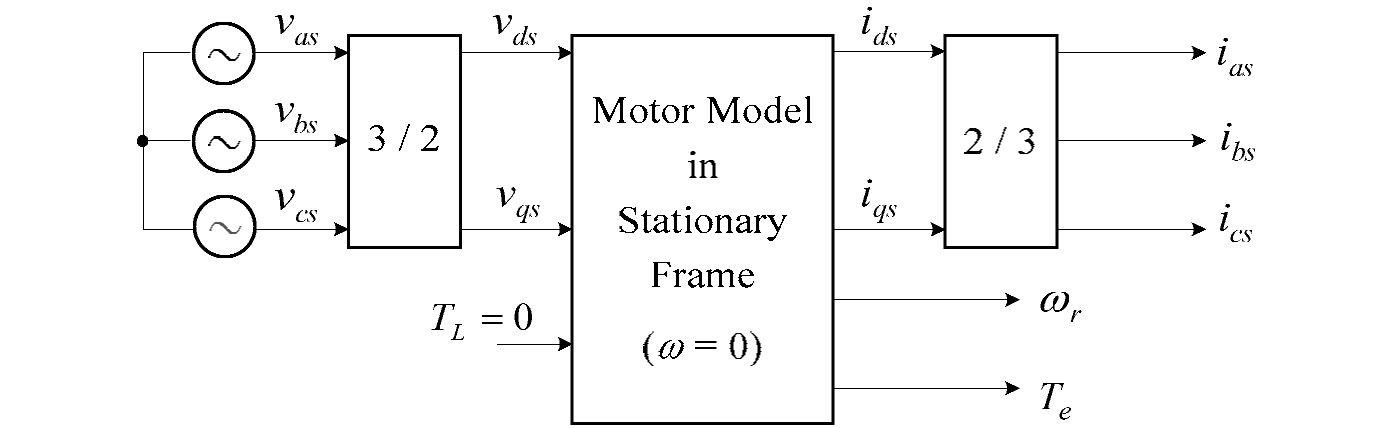
\includegraphics{graficos/img06.jpg}
\caption{Figure 14.3-4: Block diagram for simulation of motor free acceleration using the stationary-frame motor model.}
\end{figure}
\FloatBarrier

\begin{figure}[h]
\centering
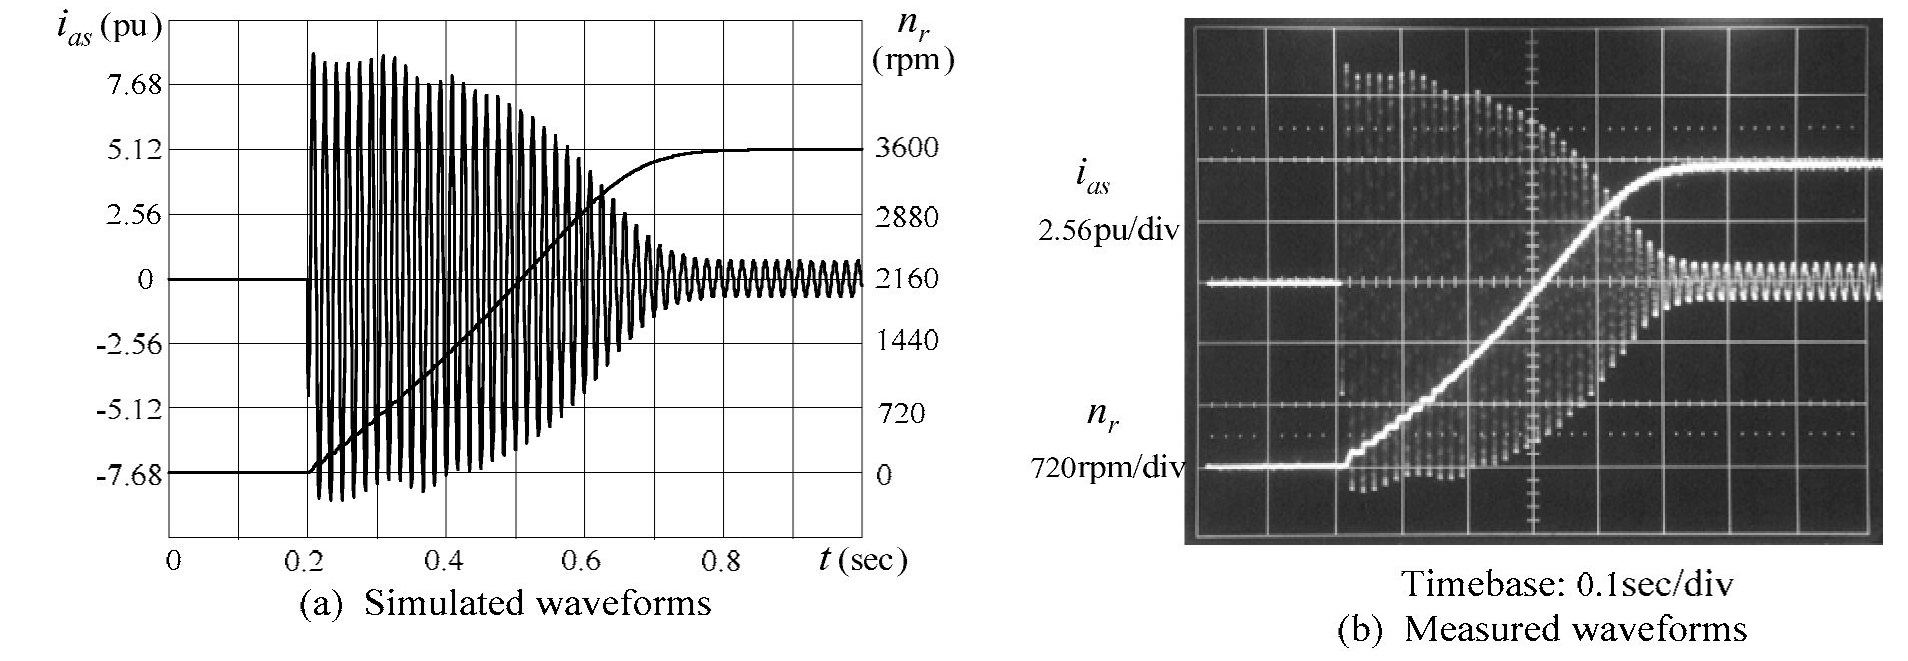
\includegraphics{graficos/img07.jpg}
\caption{Figure 14.3-5: Waveforms of an induction motor during free acceleration.}
\end{figure}
\FloatBarrier

Figure 14.3-5a shows simulated transient waveforms of the stator current $i_{as}$ and rotor speed $n_r$ during motor free acceleration (the motor starts under the rated voltage and frequency without mechanical load). The rotor speed $n_r$, in rpm relates to the angular electrical rotor speed $\omega_r$ by

\begin{equation}
n_r = \frac{30}{\pi P} \omega_r \tag{14.3-9}
\end{equation}

The peak starting current is approximately 8.4 pu, which represents the rms starting current of 5.9 pu. The starting time is around 0.5 s due to the low moment of inertia and high starting current. The measured waveforms during the free acceleration are given in Fig. 14.3-5b, which match with the simulated results very well.

\begin{figure}[h]
\centering
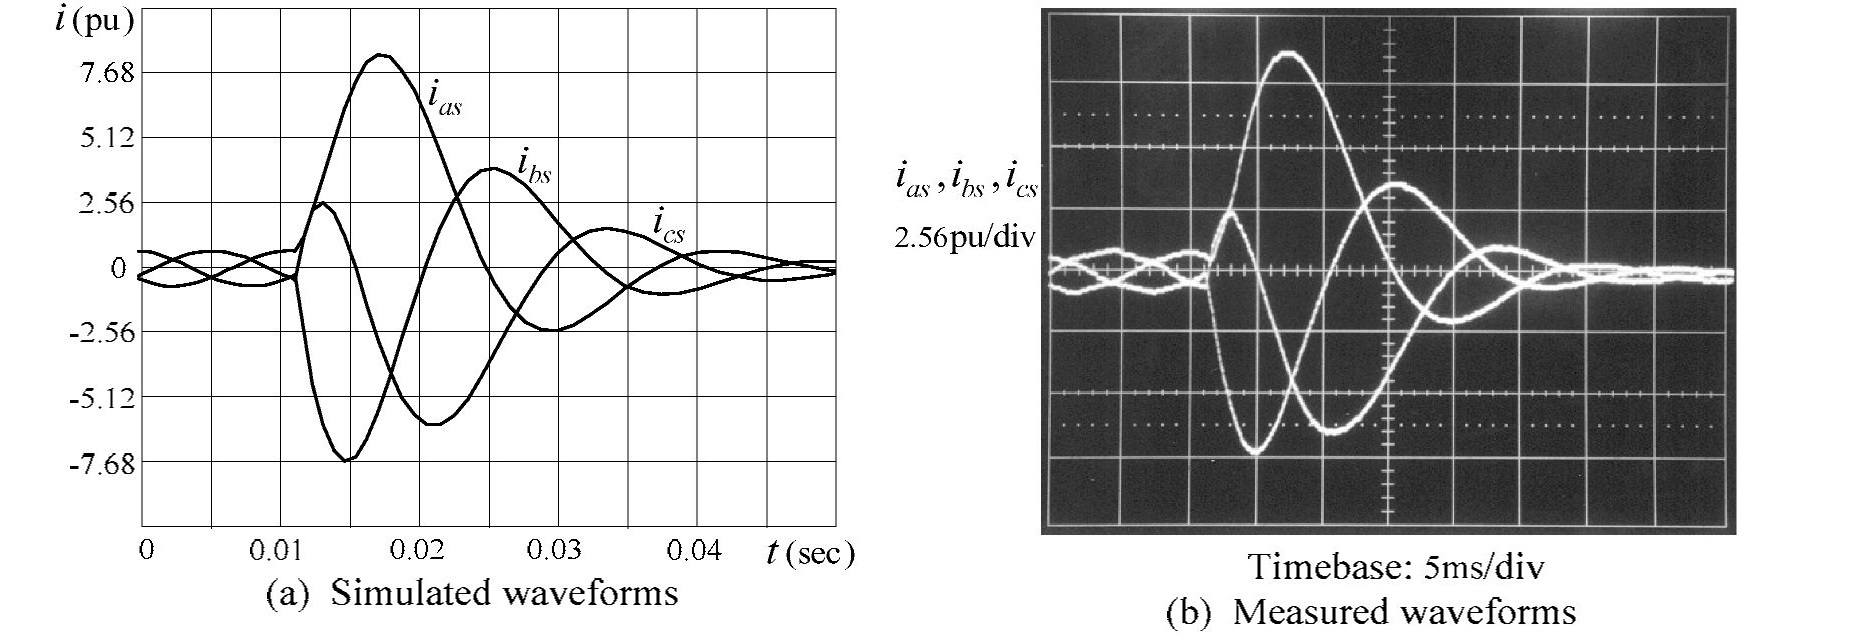
\includegraphics{graficos/img08.jpg}
\caption{Figure 14.3-6: Stator current waveforms of an induction motor during a three-phase fault.}
\end{figure}
\FloatBarrier

Figure 14.3-6 shows simulated and measured transient waveforms of the motor during a three-phase fault. The motor operates near its synchronous speed when its three-phase terminals are shorted. The maximum peak stator current is close to that during the free acceleration. The measured waveforms correlate closely with the simulated ones.

\begin{figure}[h]
\centering
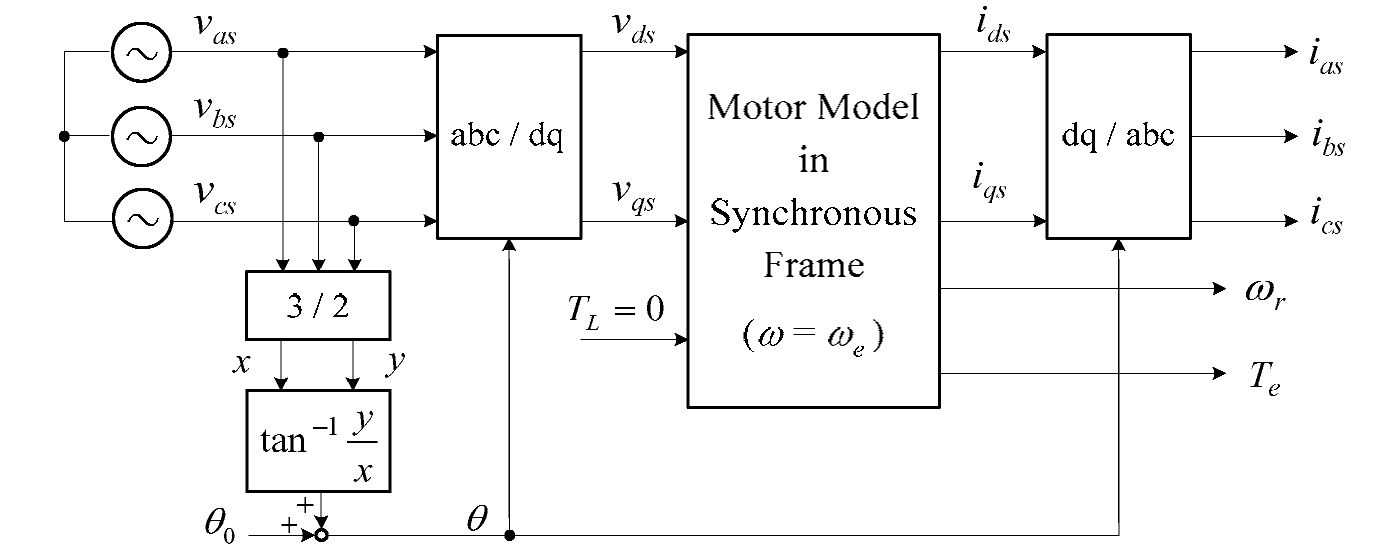
\includegraphics{graficos/img09.jpg}
\caption{Figure 14.3-7: Block diagram for simulation of motor free acceleration using the synchronous-frame motor model.}
\end{figure}
\FloatBarrier

Figure 14.3-7 illustrates the simulation block diagram with the motor model in the synchronous frame. Using the abc/dq and dq/abc transformation blocks, the three-phase supply voltages $v_{as}$, $v_{bs}$, and $v_{cs}$ in the stationary frame can be transformed to the dq-axis voltages $v_{ds}$ and $v_{qs}$ in the synchronous frame while the simulated dq-axis currents $i_{ds}$ and $i_{qs}$ in the synchronous frame can be converted to three-phase currents $i_{as}$, $i_{bs}$, and $i_{cs}$ in the stationary frame. The angle $\theta$ in the transformation blocks can be obtained by the 3/2 transformation and tan$^{-1}$ blocks shown in the figure or using Eq. (14.2-3) directly.

\begin{figure}[h]
\centering
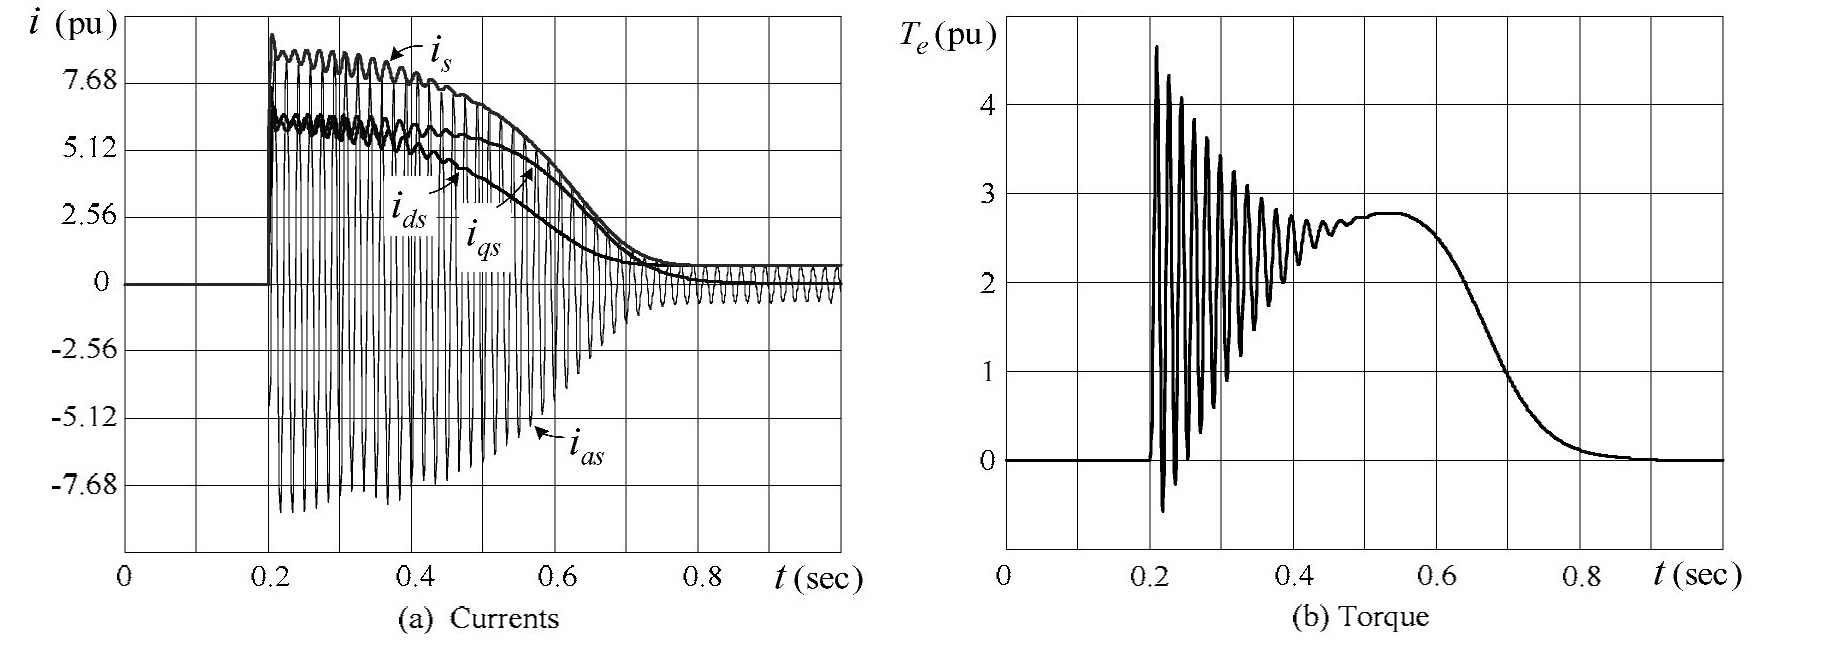
\includegraphics{graficos/img10.jpg}
\caption{Figure 14.3-8: Simulated waveforms for motor free acceleration using the synchronous-frame motor model.}
\end{figure}
\FloatBarrier

Figure 14.3-8a shows the simulated current waveforms for $i_{as}$, $i_{ds}$, and $i_{qs}$ during motor free acceleration. The waveform for $i_{as}$ in the stationary frame is exactly the same as that in Fig. 14.3-5. The dq-axis currents $i_{ds}$ and $i_{qs}$ are in the synchronous frame, and therefore they are dc signals in steady state. The amplitude of the stator current $\vec{i}_s$ can be obtained by $\vec{i}_s = \sqrt{i_{ds}^2 + i_{qs}^2}$. The dq-axis voltages $v_{ds}$ and $v_{qs}$ in the synchronous frame are of a constant dc, and therefore they are not shown in the figure.

The stator current angle $\phi$, which is the angle between $\vec{i}_s$ and the d-axis as shown in Fig. 14.2-2b, will affect waveforms for $i_{ds}$ and $i_{qs}$. The waveforms in Fig. 14.3-8a are obtained with $\phi = 0$ by adjusting the initial angle $\theta_0$ such that the d-axis of the synchronous frame is aligned with $\vec{i}_s$. This leads to $i_{qs} = 0$ and $i_{ds} = i_s$ when the motor is in steady-state operation. If the q-axis of the synchronous frame is aligned with $\vec{i}_s$ ($\phi = 90^\circ$), the steady-state dq-axis currents are $i_{qs} = i_s$ and $i_{ds} = 0$. However, the waveform for $i_s$ is not affected by $\phi$.

The torque response during the motor free acceleration is shown in Fig. 14.3-8b. Although it is obtained with the motor model in the synchronous frame, the response remains the same for the motor model in any other reference frames.

\clearpage
\section{Principle of Field-Oriented Control (FOC)}

\subsection{Field Orientation}

It is well known that the dc motor drive has an excellent dynamic performance. This is mainly due to the decoupled (separate) control of stator magnetic field and electromagnetic torque of the motor. The torque is developed by the interaction of two perpendicular magnetic fields. One field is generated by the field current $i_f$ in the stator winding, and the other is produced by the armature (rotor) current $i_a$. The developed torque can be expressed as

\begin{equation}
T_e = K_a \lambda_f i_a \tag{14.4-1}
\end{equation}

where $K_a$ is an armature constant and $\lambda_f$ is the flux produced by $i_f$. In high-performance dc drives, $\lambda_f$ is normally kept constant by keeping $i_f$ constant, and thus the torque $T_e$ is proportional to and can be directly controlled by $i_a$.

The field-oriented control, also known as vector control, for induction motor emulates the dc motor control. Using a proper field orientation, the stator current can be decomposed into a flux-producing component and a torque-producing component. These two components are then controlled separately.

The field orientation can be generally classified into stator flux, air-gap flux, and rotor flux orientations [3, 4]. Since the rotor flux orientation is extensively used in ac drives, this scheme is to be analyzed in detail. Its operating principle can be easily applied to the other two field orientation schemes.

\begin{figure}[h]
\centering
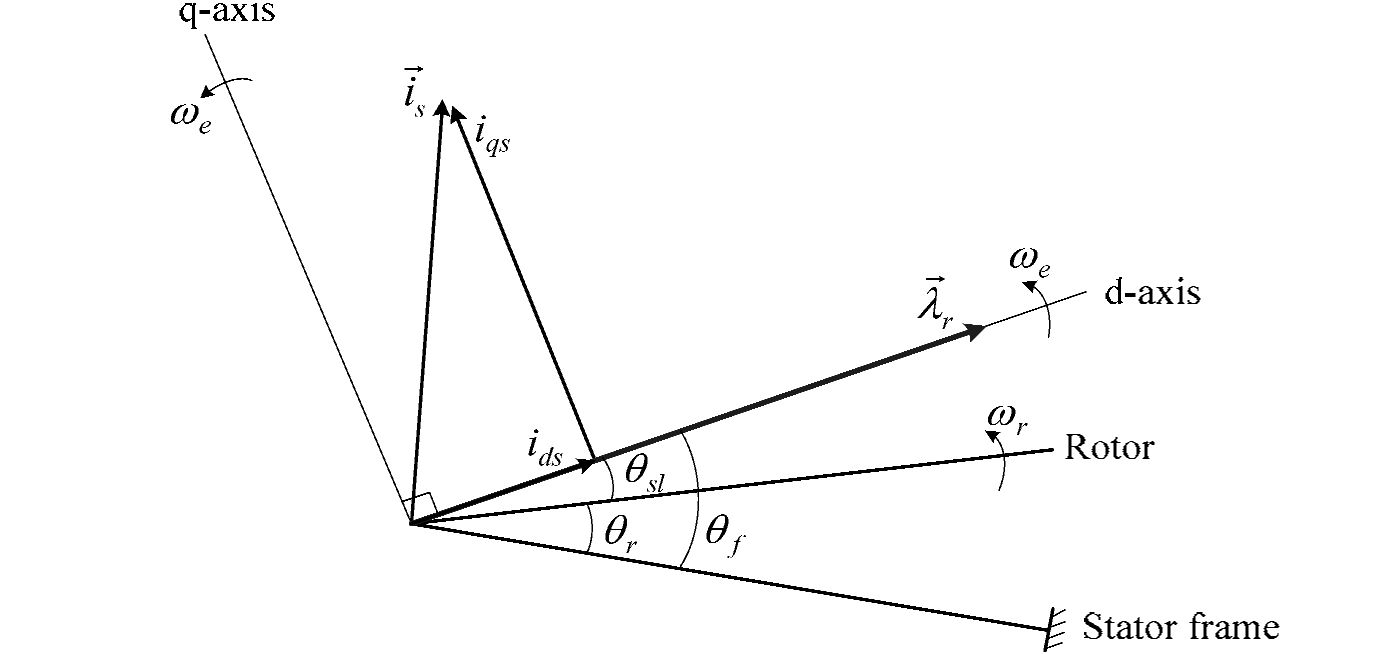
\includegraphics{graficos/img11.jpg}
\caption{Figure 14.4-1: Rotor flux field orientation (the d-axis is aligned with $\vec{\lambda}_r$).}
\end{figure}
\FloatBarrier

The rotor flux orientation is achieved by aligning the d-axis of the synchronous reference frame with the rotor flux vector $\vec{\lambda}_r$ as shown in Fig. 14.4-1. The resultant d- and q-axis rotor flux components are

\begin{equation}
\lambda_{qr} = 0 \quad \text{and} \quad \lambda_{dr} = \lambda_r \tag{14.4-2}
\end{equation}

where $\lambda_r$ is the magnitude of $\vec{\lambda}_r$. Substituting (14.4-2) into the last equation of (14.3-8) yields

\begin{equation}
T_e = K_r \lambda_r i_{qs} = K_r \lambda_r i_{qs} \tag{14.4-3}
\end{equation}

where $K_r = 3PL_m/2L_r$. Equation (14.4-3) indicates that with the rotor field orientation the torque expression for the induction motor is similar to that of a dc motor. If $\lambda_r$ can be kept constant during the motor operation, the developed torque can be directly controlled by the q-axis stator current $i_{qs}$.

The stator current vector $\vec{i}_s$ in Fig. 14.4-1 can be resolved into two components along the dq-axes. The d-axis current $i_{ds}$ is referred to as flux-producing current while the q-axis current $i_{qs}$, which is perpendicular to $i_{ds}$, is the torque-producing current. In the field-oriented control, $i_{ds}$ is normally kept at its rated value while $i_{qs}$ is controlled independently. With the decoupled control for $i_{ds}$ and $i_{qs}$, a high-performance drive can be realized.

One of the key issues associated with the rotor flux-oriented control is to accurately determine the rotor flux angle $\theta_f$ for field orientation. Various schemes can be used to find $\theta_f$. For instance, it can be calculated from measured stator voltages and currents, or it can be found from

\begin{equation}
\theta_f = \theta_r + \theta_{sl} \tag{14.4-4}
\end{equation}

where $\theta_r$ and $\theta_{sl}$ are the measured rotor position angle and calculated slip angle, respectively.

\subsection{General Block Diagram of FOC}

Depending on how the rotor flux angle $\theta_f$ is obtained, the control schemes can be classified into direct and indirect field-oriented controls. If $\theta_f$ is obtained by using flux-sensing devices embedded inside the motor or using measured motor terminal voltages and currents, the method is referred to as direct field-oriented control. If the rotor flux angle $\theta_f$ is obtained from detected rotor position angle $\theta_r$ and calculated slip angle $\theta_{sl}$ as shown in (14.4-4), this scheme is known as \textit{indirect field-oriented control} [3, 4].

\begin{figure}[h]
\centering
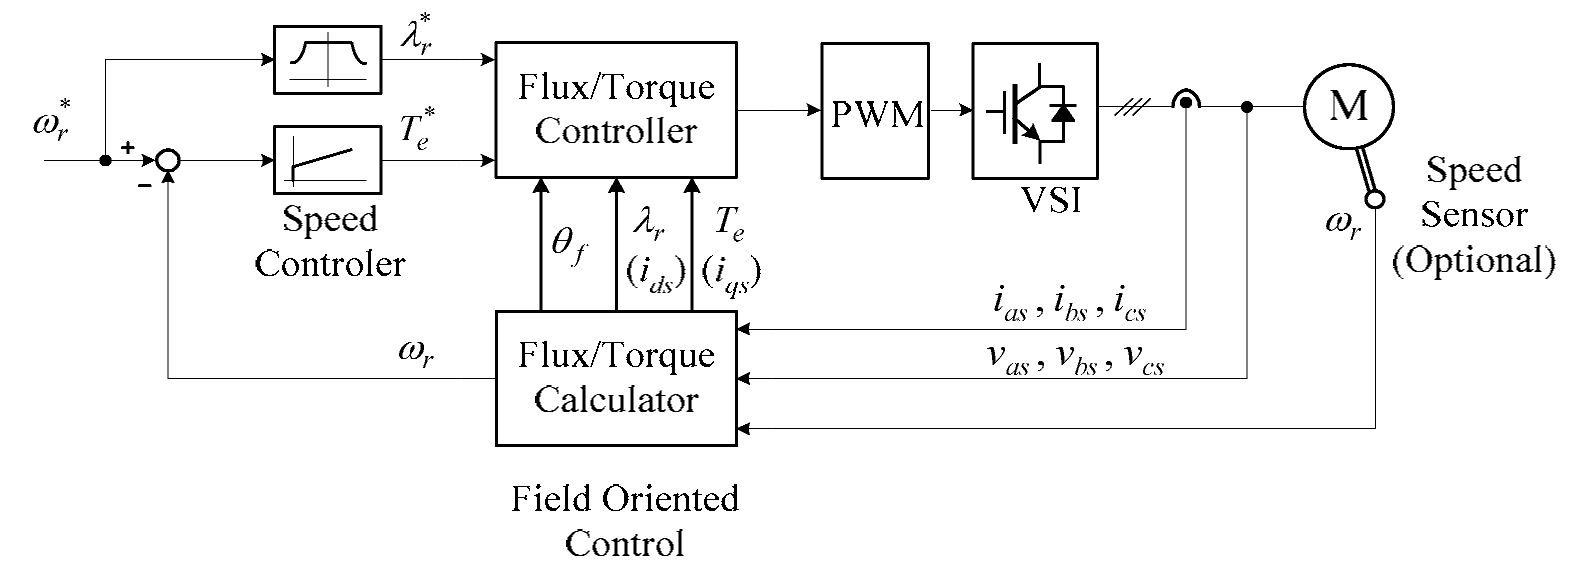
\includegraphics{graficos/img12.jpg}
\caption{Figure 14.4-2: General block diagram of rotor flux FOC.}
\end{figure}
\FloatBarrier

A general block diagram of an induction motor drive with rotor flux-oriented control is shown in Fig. 14.4-2. Since the essence of the FOC is the decoupled control of the rotor flux $\lambda_r$ and electromagnetic torque $T_e$, these two variables are controlled separately. The torque reference $T_e^*$ is generated by \textit{Speed Controller} based on the reference speed $\omega_r^*$ and the detected or estimated rotor speed $\omega_r$. The rotor flux reference $\lambda_r^*$ is a function of $\omega_r^*$. When the motor operates at or below its rated speed, $\lambda_r^*$ is normally kept at its rated value. With the rated speed exceeded, $\lambda_r^*$ should be weakened accordingly such that the stator voltage and the output power of the motor would not exceed their ratings.

The two references $\lambda_r^*$ and $T_e^*$ are then sent to \textit{Flux/Torque Controller}, where they are compared with calculated rotor flux $\lambda_r$ and torque $T_e$ for a closed-loop control. The \textit{Flux/Torque Controller} generates reference signals for the PWM block, which produces gate signals for the inverter to adjust its output voltage and frequency.

Based on the measured stator voltage and current variables and the motor model, the \textit{Flux/Torque Calculator} calculates (1) the rotor flux angle $\theta_f$ for field orientation, (2) the rotor flux magnitude $\lambda_r$, or the flux-producing current $i_{ds}$, (3) the electromagnetic torque $T_e$ or the torque-producing current $i_{qs}$, and (4) the rotor speed $\omega_r$. Depending on drive system requirements and the type of the FOC scheme employed, the rotor speed $\omega_r$ may also be directly detected by a digital speed sensor. It is worth noting that the \textit{Flux/Torque Calculator}, also known as \textit{Flux/Torque Observer} or \textit{Estimator} in the literature, is the most important functional block in the FOC scheme.

\clearpage
\section{Direct Field-Oriented Control}

\subsection{System Block Diagram}

\begin{figure}[h]
\centering
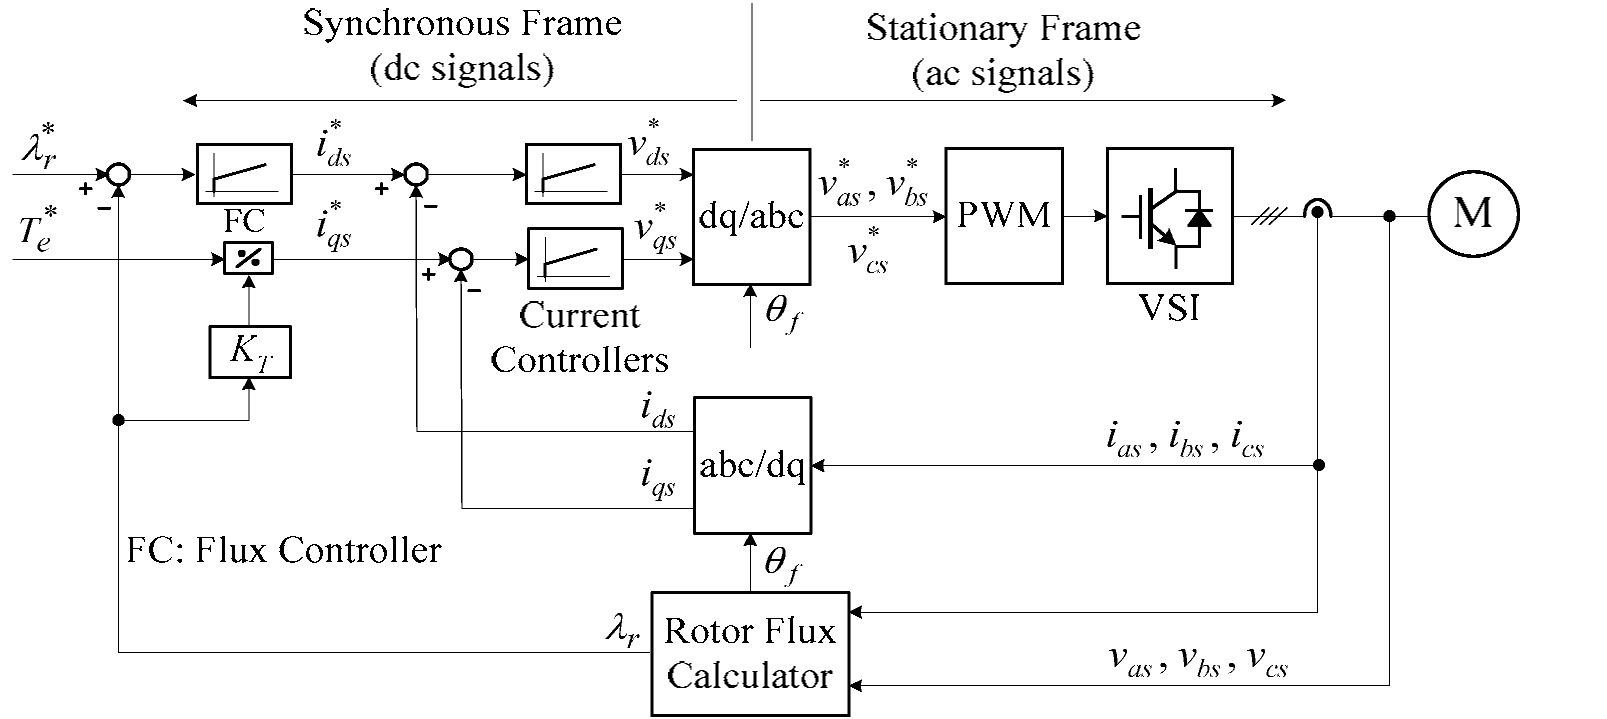
\includegraphics{graficos/img13.jpg}
\caption{Figure 14.5-1: Direct field-oriented control with rotor flux orientation.}
\end{figure}
\FloatBarrier

Figure 14.5-1 shows a typical block diagram of direct field-oriented control for induction motor, where the rotor speed control is not shown for simplicity. There are three feedback control loops, one for the rotor flux linkage $\lambda_r$, one for the d-axis (flux-producing) stator current $i_{ds}$, and another for the q-axis (torque-producing) stator current $i_{qs}$.

For the rotor flux control, the calculated $\lambda_r$ is compared with its reference $\lambda_r^*$ to generate the d-axis stator current reference $i_{ds}^*$ through flux controller (FC). The q-axis stator current reference $i_{qs}^*$ is generated according to the torque reference $T_e^*$. The feedback dq-axis stator currents $i_{ds}$ and $i_{qs}$ are compared with their references, and the errors are sent to current controllers to generate stator voltage references $v_{ds}^*$ and $v_{qs}^*$. The dq-axis voltages in the synchronous frame are then transformed to the three-phase stator voltages $v_{as}^*$, $v_{bs}^*$, and $v_{cs}^*$ in the stationary frame for the PWM block. Various PWM schemes can be used. If a carrier-based modulation scheme is employed, $v_{as}^*$, $v_{bs}^*$, and $v_{cs}^*$ are the modulating signals that are compared with a triangular carrier wave to generate PWM gating for the switching devices in the inverter.

As shown in Fig. 14.5-1, the rotor flux angle $\theta_f$ is used in the abc/dq and dq/abc transformation blocks for field orientation. The variables to the left of the transformation blocks are all dc signals in the synchronous frame, while those on the right side of the transformation blocks are all ac variables in the stationary frame.

\subsection{Rotor Flux Calculator}

Based on the stationary-frame motor model in Fig. 14.3-2b, the stator flux vector can be expressed as

\begin{equation}
\vec{\lambda}_s = \int (\vec{v}_s - R_s \vec{i}_s) \, dt \tag{14.5-1}
\end{equation}

The rotor flux vector can be found from the flux-linkage equations (14.3-2):

\begin{equation}
\vec{\lambda}_r = L_r \frac{\vec{\lambda}_s - L_s \vec{i}_s}{L_m} + L_m \vec{i}_s = \frac{L_r}{L_m} (\vec{\lambda}_s - \sigma L_s \vec{i}_s) \tag{14.5-2}
\end{equation}

where $\sigma$ is the total leakage factor, defined by

\begin{equation}
\sigma = 1 - \frac{L_m^2}{L_s L_r} \tag{14.5-3}
\end{equation}

Decomposing the rotor flux $\vec{\lambda}_r$ into the d- and q-axis components, we have

\begin{equation}
\lambda_{dr} = \frac{L_r}{L_m} (\lambda_{ds} - \sigma L_s i_{ds}) \tag{14.5-4}
\end{equation}
\begin{equation}
\lambda_{qr} = \frac{L_r}{L_m} (\lambda_{qs} - \sigma L_s i_{qs}) \tag{14.5-4}
\end{equation}

from which the magnitude and angle of the rotor flux are

\begin{equation}
\lambda_r = \sqrt{\lambda_{dr}^2 + \lambda_{qr}^2} \tag{14.5-5}
\end{equation}
\begin{equation}
\theta_r = \tan^{-1} \frac{\lambda_{qr}}{\lambda_{dr}} \tag{14.5-5}
\end{equation}

The following can be noted from (14.5-1) to (14.5-5):

\begin{itemize}
    \item The rotor flux magnitude $\lambda_r$ and its angle $\theta_r$ can be identified based on measured stator voltage $\vec{v}_s$, stator current $\vec{i}_s$ and motor parameters ($L_s$, $L_r$, $L_m$ and $R_s$).
    \item Since the stationary-frame motor model is used, all the variables such as $\lambda_{dr}$, $\lambda_{qr}$, $i_{ds}$, and $i_{qs}$ (except $\lambda_r$ and $\theta_r$) are of ac signals. Neglecting the switching harmonics, they are sinusoidal in steady state.
\end{itemize}

\begin{figure}[h]
\centering
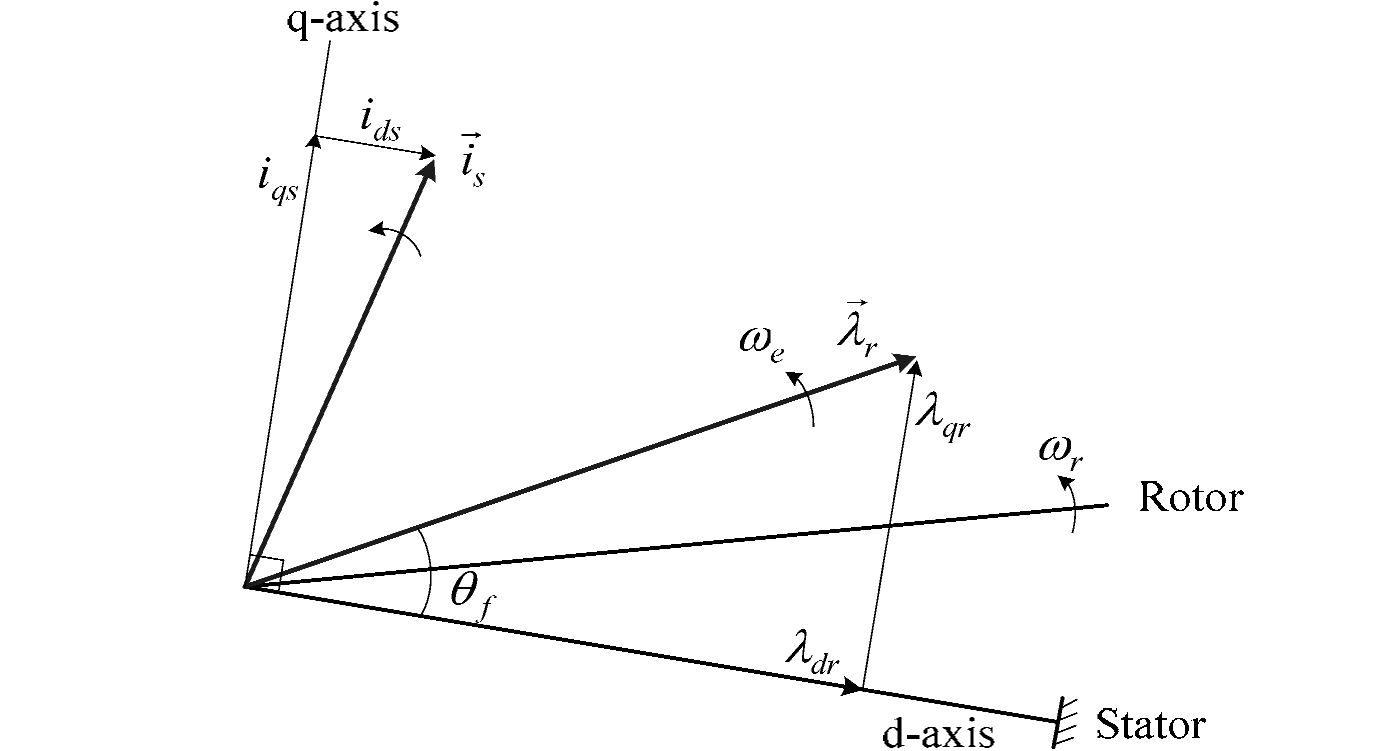
\includegraphics{graficos/img14.jpg}
\caption{Figure 14.5-2: Vector diagram for $\vec{\lambda}_r$ and $\vec{i}_s$ used in rotor flux calculator.}
\end{figure}
\FloatBarrier

Figure 14.5-2 shows the vector diagram for the rotor flux vector $\vec{\lambda}_r$ and stator current vector $\vec{i}_s$ used in the Rotor Flux Calculator. When the two vectors rotate one revolution in space, their dq-axis components $\lambda_{dr}$, $\lambda_{qr}$, $i_{ds}$, and $i_{qs}$ in the stationary (stator) frame vary one cycle over time.

\begin{figure}[h]
\centering
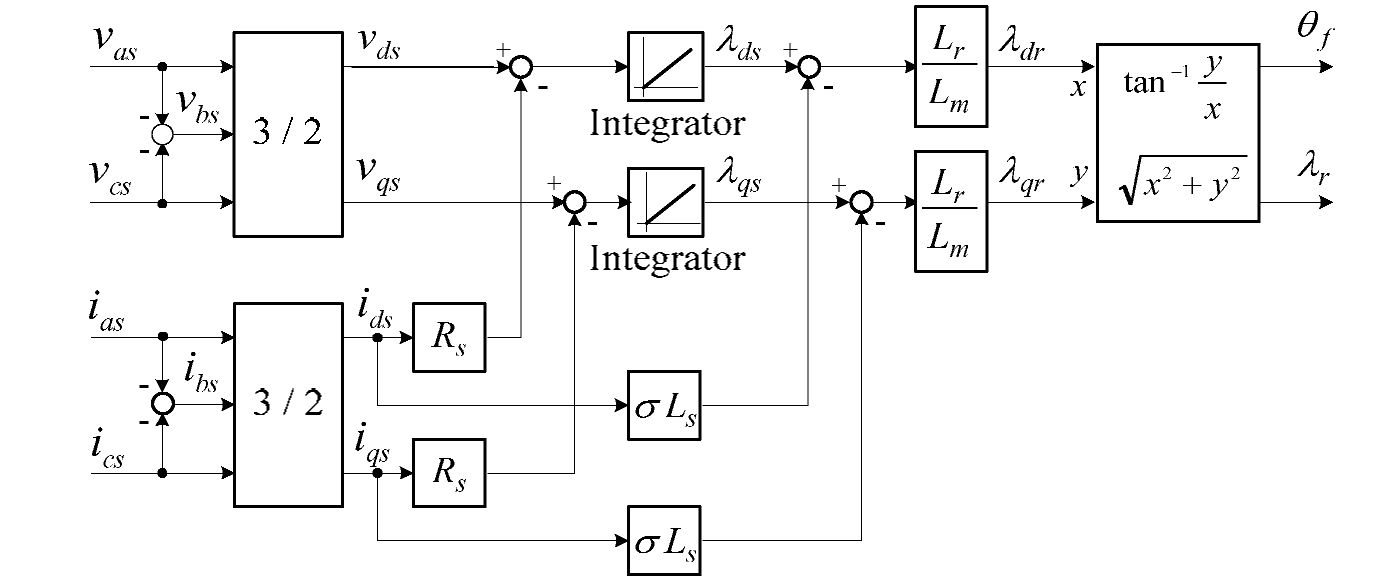
\includegraphics{graficos/img15.jpg}
\caption{Figure 14.5-3: Block diagram for the rotor flux calculation.}
\end{figure}
\FloatBarrier

Figure 14.5-3 shows the block diagram for the digital implementation of Rotor Flux Calculator. Of the three stator voltages $v_{as}$, $v_{bs}$, and $v_{cs}$, only two need to be measured and the third one can be found from $v_{as} + v_{bs} + v_{cs} = 0$. To reduce the number of voltage sensors, the stator voltages can also be reconstructed by using the inverter switching function and measured dc voltage. The stator voltages and currents are then transformed to two-phase variables through 3/2 stationary transformation blocks. The other blocks are derived from equations (14.5-1) to (14.5-5). The output of the Rotor Flux Calculator is the rotor flux angle $\theta_f$ and its amplitude $\lambda_r$.

\subsection{Direct FOC with Current-Controlled VSI}

\begin{figure}[h]
\centering
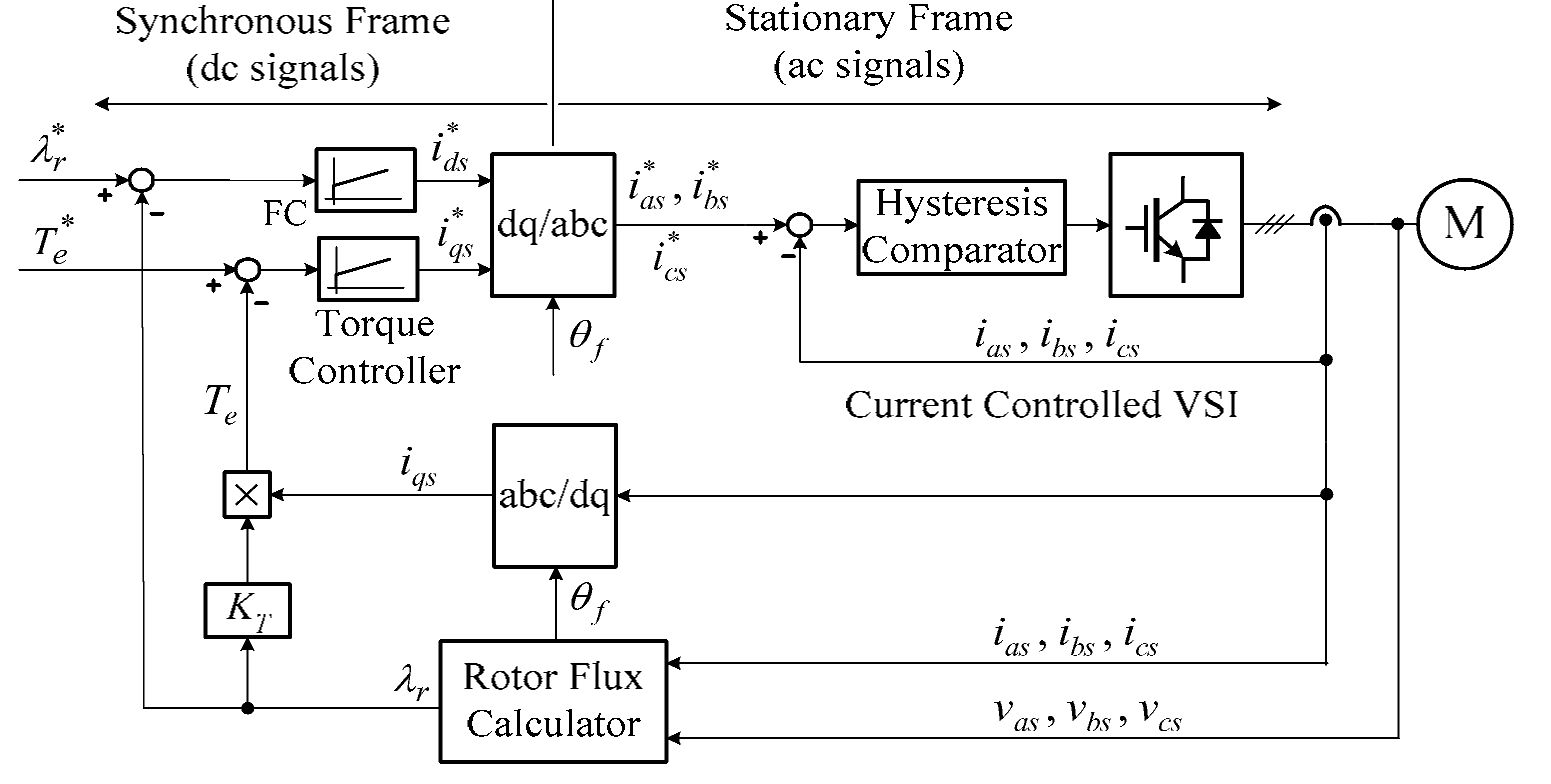
\includegraphics[scale=0.9]{graficos/img16.jpg}
\caption{Figure 14.5-4: Direct FOC with a current regulated VSI.}
\end{figure}
\FloatBarrier

The direct FOC scheme discussed in the previous sections can be simplified if a current-regulated voltage source inverter is used. Figure 14.5-4 shows the block diagram of such a system. The current-regulated VSI can make the inverter output currents $i_{as}$, $i_{bs}$ and $i_{cs}$ follow their references $i_{as}^*$, $i_{bs}^*$, and $i_{cs}^*$ closely. Therefore,there is no need to use the current controllers in Fig. 14.5-1. Furthermore, the PWM scheme for the current regulated VSI is simpler than other modulation techniques.

\begin{figure}[h]
\centering
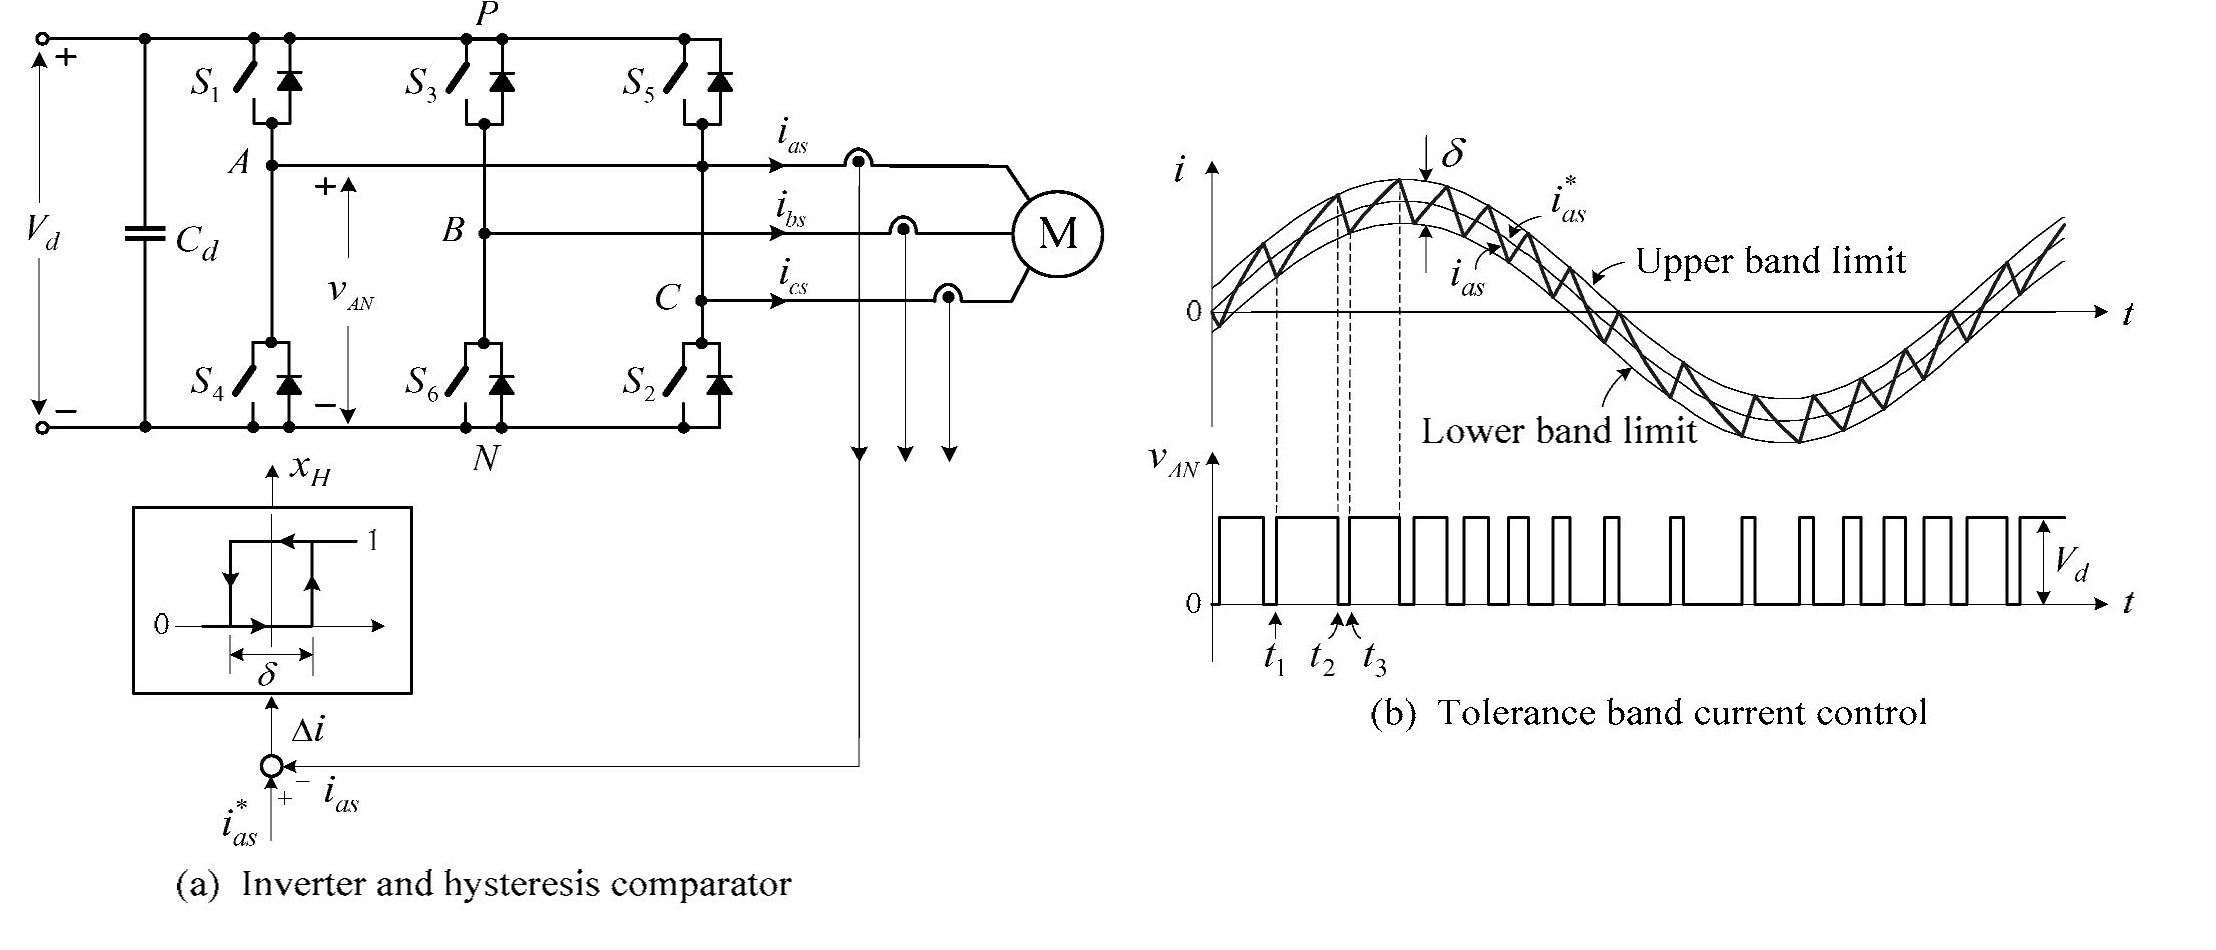
\includegraphics[scale=0.8]{graficos/img17.jpg}
\caption{Figure 14.5-5: Current-regulated voltage source inverter.}
\end{figure}
\FloatBarrier

The operating principle of the current regulated VSI is illustrated in Fig. 14.5-5, where the control of only one of the three phase currents is shown. The inverter output current $i_{as}$ is measured and compared with its reference $i_{as}^*$. Their difference $\Delta i$ is sent to a hysteresis comparator. The output of the comparator $x_H$ is either logic ‘1’ or ‘0’, based on which gate signals are generated for switches $S_1$ and $S_4$. The hysteresis comparator has a tolerance band of $\delta$.

Assume that the reference current $i_{as}^*$ is sinusoidal as illustrated in Fig. 14.5-5b. The inverter output current $i_{as}$ is confined within the upper and lower band limits set by $\delta$. Assuming that $x_H$ becomes logic ‘1’ at time instant $t_1$, $S_1$ is turned on and $S_4$ is turned off. The inverter terminal voltage $v_{AN}$ is equal to the dc voltage $V_d$, causing $i_{as}$ to increase. The rate of current rise is mainly determined by $V_d$, motor parameters and its back emf. When $i_{as}$ reaches its upper band limit at $t_2$, $x_H$ becomes logic ‘0’, leading to the turn-off of $S_1$ and turn-on of $S_4$. The resultant $v_{AN}$ is zero, causing $i_{as}$ to decrease. When $i_{as}$ hits the lower band limit at $t_3$, $x_H$ = ‘0’, $v_{AN}$ = $V_d$, and $i_{as}$ starts to increase again. As a result, $i_{as}$ is kept within the upper and lower band limits. To make $i_{as}$ follow its reference $i_{as}^*$ more closely with less switching harmonics, the bandwidth $\delta$ can be reduced. However, this is accomplished at the expense of an increased switching frequency.

For a given $\delta$ and $V_d$, the inverter switching frequency may vary with motor parameters. This is considered as a major drawback of the current-regulated inverter with the tolerance band control. When the inverter uses other modulation techniques such as SPWM and SVM, its switching frequency is set by the modulation scheme, independent of motor parameters.

\begin{figure}[h]
\centering
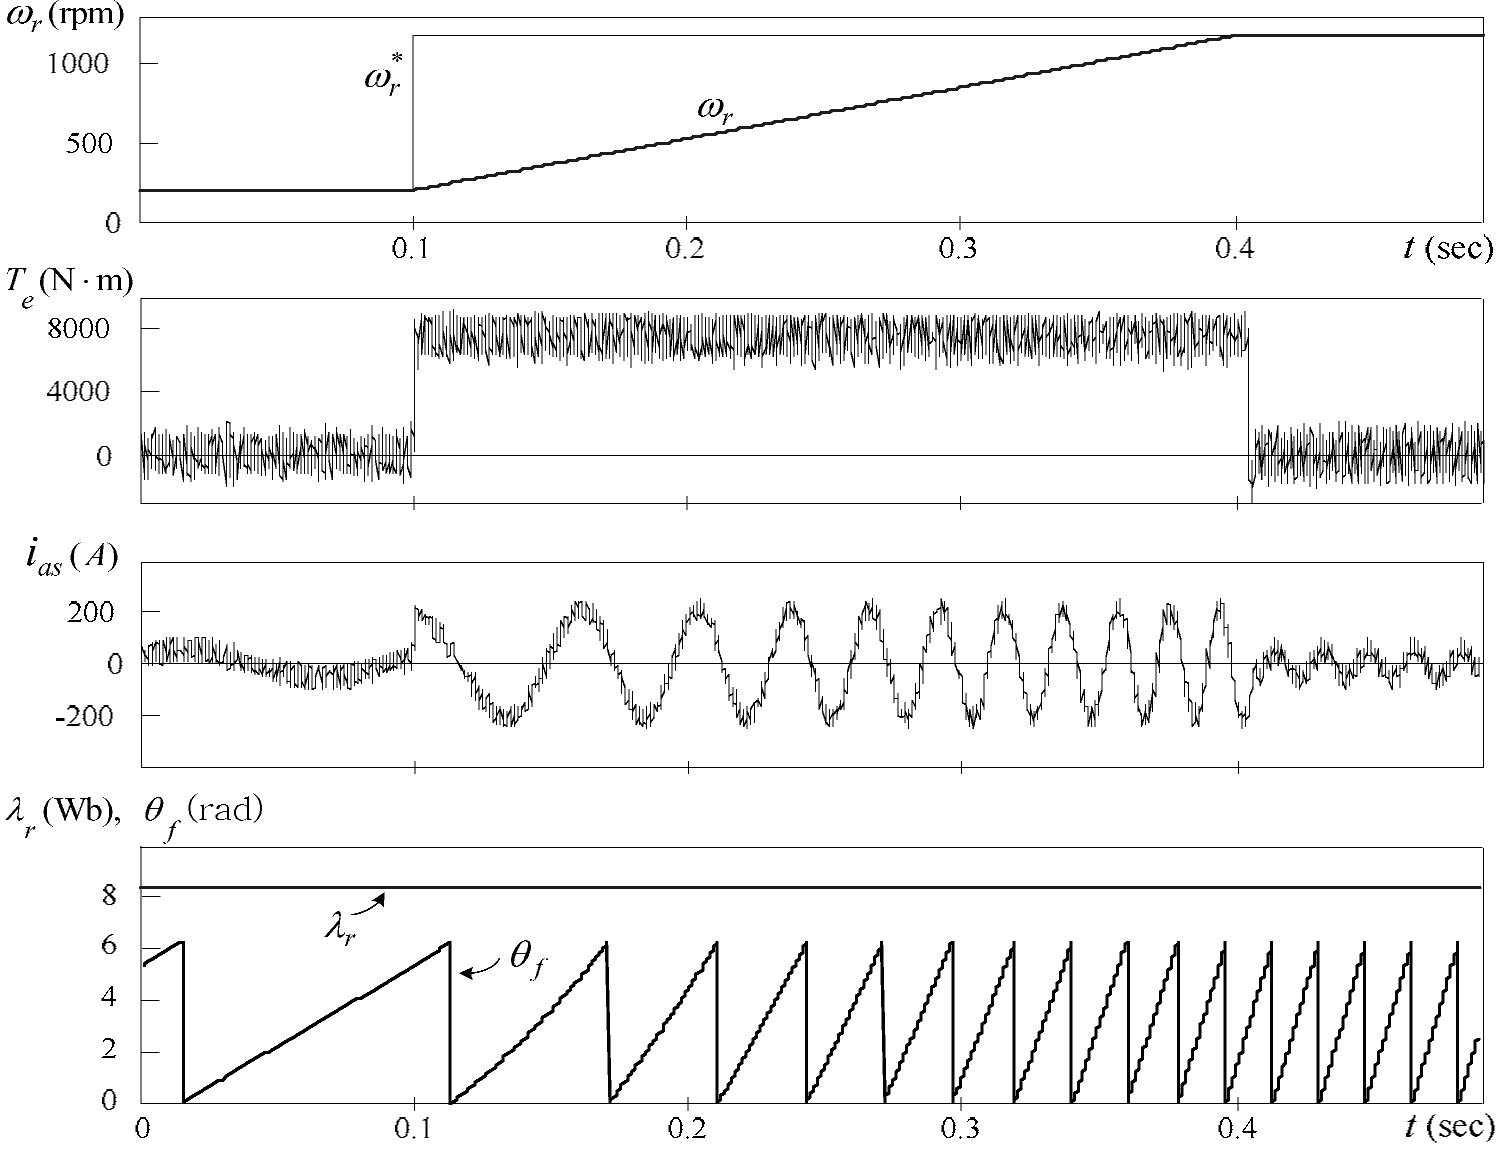
\includegraphics[scale=0.8]{graficos/img18.jpg}
\caption{Figure 14.5-6: Simulated waveforms for an induction motor drive with direct FOC scheme.}
\end{figure}
\FloatBarrier

Figure 14.5-6 shows the simulated waveforms for an induction motor drive using the direct FOC scheme. The block diagram of the drive system is shown Fig. 14.5-4, where the speed control loop is not shown. The motor nameplate data and parameters are listed in Table 14.5-1.

The tolerance band $\delta$ of the hysteresis comparator is adjusted such that inverter switching frequency is around 600 Hz. The rotor flux reference $\lambda_r^*$ is set to its rated value of 8.35 Wb. The maximum torque is limited to its rated value of 7490 N·m during motor transients.

The motor initially operates at a rotor speed of $n_r = 200$ rpm. The speed reference $n_r^*$ has a step increase from 200 rpm to the rated rotor speed of 1189 rpm at time instant of $t = 0.1$ s. The motor accelerates under the no-load condition while its torque is limited to the rated value. The torque contains high ripples due to the low switching frequency. The stator current $i_{as}$ rises to its rated value during the transient. When $n_r$ reaches its reference of 1189 rpm around $t = 0.4$ s, the average $T_e$ drops to zero, and $i_{as}$ reduces to a value that corresponds to the magnetizing current of the motor. Due to the decoupled flux and torque control by the FOC scheme, the rotor flux magnitude $\lambda_r$ is kept constant during transients. The rotor flux angle $\theta_f$ is also given in the figure.

\section{Indirect Field-Oriented Control}

\begin{figure}[h]
\centering
\caption{Table 14.5-1: Motor Nameplate and Parameters.}
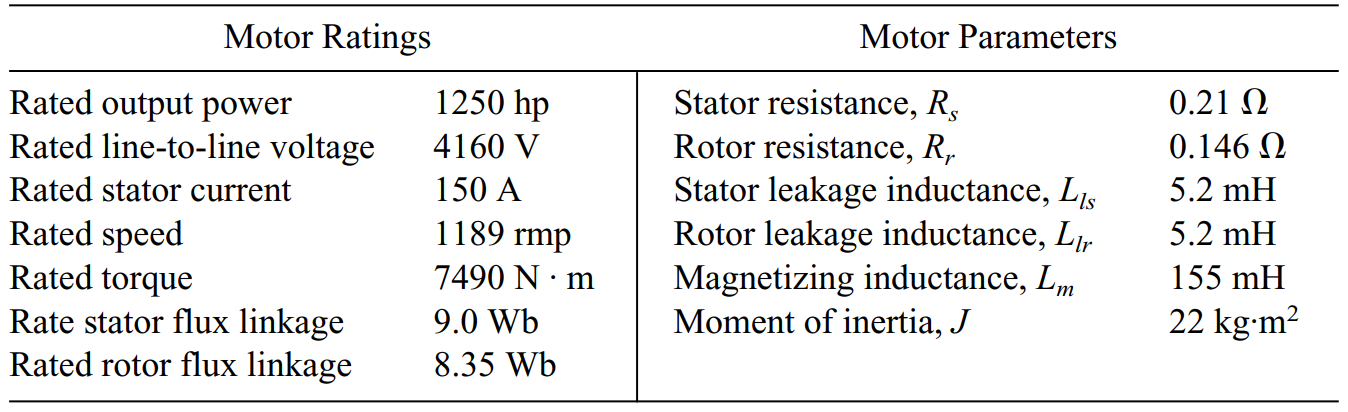
\includegraphics[scale=0.4]{graficos/tabla_14_5_1.png}
\end{figure}
\FloatBarrier

\begin{figure}[h]
\centering
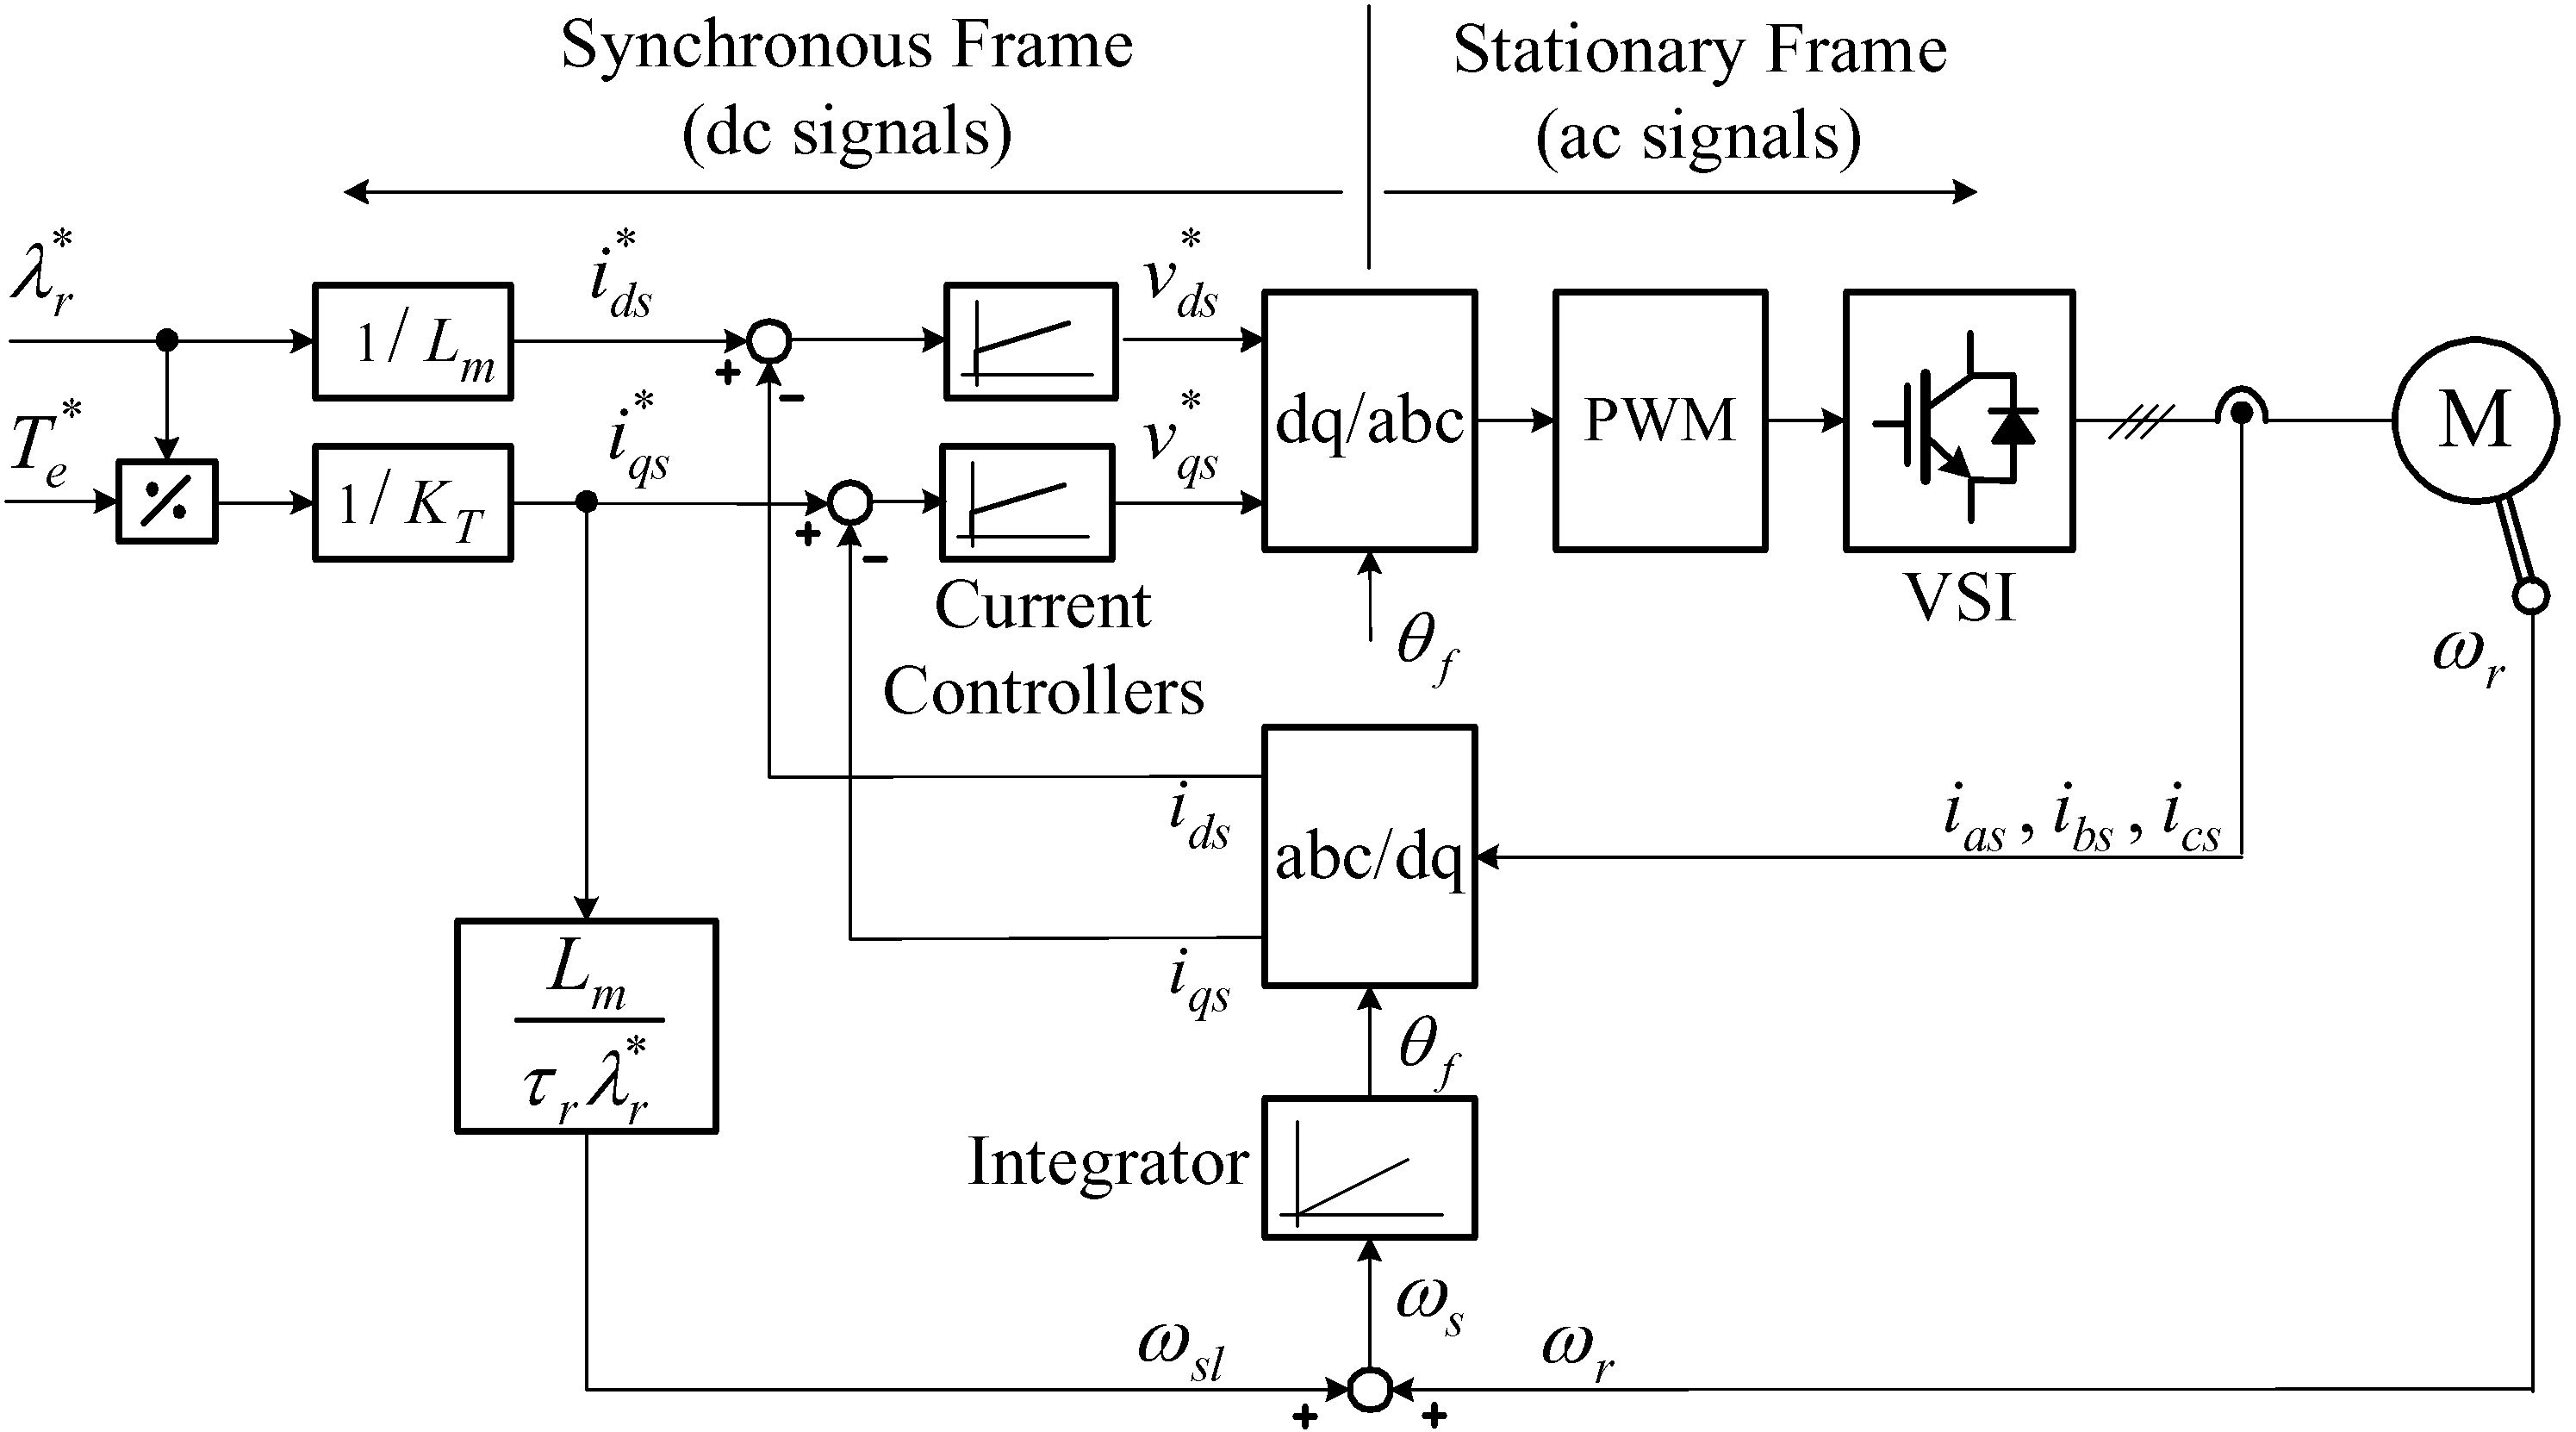
\includegraphics{graficos/img19.jpg}
\caption{Figure 14.6-1: Indirect field-oriented control with rotor flux orientation.}
\end{figure}
\FloatBarrier

A digital rotor speed sensor is required for indirect field-oriented control schemes. The rotor flux angle $\theta_f$ for field orientation is obtained from the measured rotor speed and calculated slip angle based on motor parameters. A typical block diagram of the indirect FOC is shown in Fig. 14.6-1. Since the rotor speed $\omega_r$ is directly measured, the rotor flux angle $\theta_f$ can be found from

\begin{equation}
\theta_f = \int (\omega_r + \omega_{sl}) \, dt \tag{14.6-1}
\end{equation}

where $\omega_{sl}$ is the angular slip frequency.

The slip frequency $\omega_{sl}$ can be derived from the synchronous-frame motor model of Fig. 14.3-2a, from which

\begin{equation}
p \lambda_r = -R_r \vec{i}_r - j \omega_{sl} \vec{\lambda}_r \tag{14.6-2}
\end{equation}

Substituting the rotor current

\begin{equation}
\vec{i}_r = \frac{1}{L_r} (\vec{\lambda}_r - L_m \vec{i}_s) \tag{14.6-3}
\end{equation}

into (14.6-2) yields

\begin{equation}
p \vec{\lambda}_r = -\frac{R_r}{L_r} \left( \vec{\lambda}_r - L_m \vec{i}_s \right) - j \omega_{sl} \vec{\lambda}_r \tag{14.6-4}
\end{equation}

from which

\begin{equation}
\vec{\lambda}_r (1 + \tau_r (p + j \omega_{sl})) = L_m \vec{i}_s \tag{14.6-5}
\end{equation}

where $\tau_r$ is the rotor time constant, defined by

\begin{equation}
\tau_r = \frac{L_r}{R_r} \tag{14.6-6}
\end{equation}

Decomposing (14.6-5) into the $dq$-axis components and taking into account the rotor flux orientation ($j \lambda_{qr} = 0$ and $\lambda_{dr} = \lambda_r$), we have

\begin{equation}
\lambda_r (1 + p \tau_r) = L_m i_{ds} \tag{14.6-7}
\end{equation}

\begin{equation}
\omega_{sl} \tau_r \lambda_r = L_m i_{qs} \tag{14.6-7}
\end{equation}

from which

\begin{equation}
\omega_{sl} = \frac{L_m}{\tau_r \lambda_r} i_{qs} \tag{14.6-8}
\end{equation}

As shown in Fig. 14.6-1, the rotor flux and torque are controlled by two feedback loops separately. Based on (14.6-7), the relationship between the rotor flux reference $\lambda_r^*$ and d-axis current reference $i_{ds}^*$ can be expressed as

\begin{equation}
i_{ds}^* = \frac{(1 + p \tau_r)}{L_m} \lambda_r^* \tag{14.6-9}
\end{equation}

Since $\lambda_r^*$ is normally kept constant during operation ($p \lambda_r^* = 0$), (14.6-9) can be simplified to

\begin{equation}
i_{ds}^* = \frac{1}{L_m} \lambda_r^* \tag{14.6-10}
\end{equation}

The q-axis current reference $i_{qs}^*$ can be obtained from the torque equation of (14.4-3):

\begin{equation}
i_{qs}^* = \frac{1}{K_T \lambda_r^*} T_e^* \tag{14.6-11}
\end{equation}

For a given $\lambda_r^*$, the torque-producing current $i_{qs}^*$ is proportional to $T_e^*$.

\section{FOC for CSI-Fed Drives}

\begin{figure}[h]
\centering
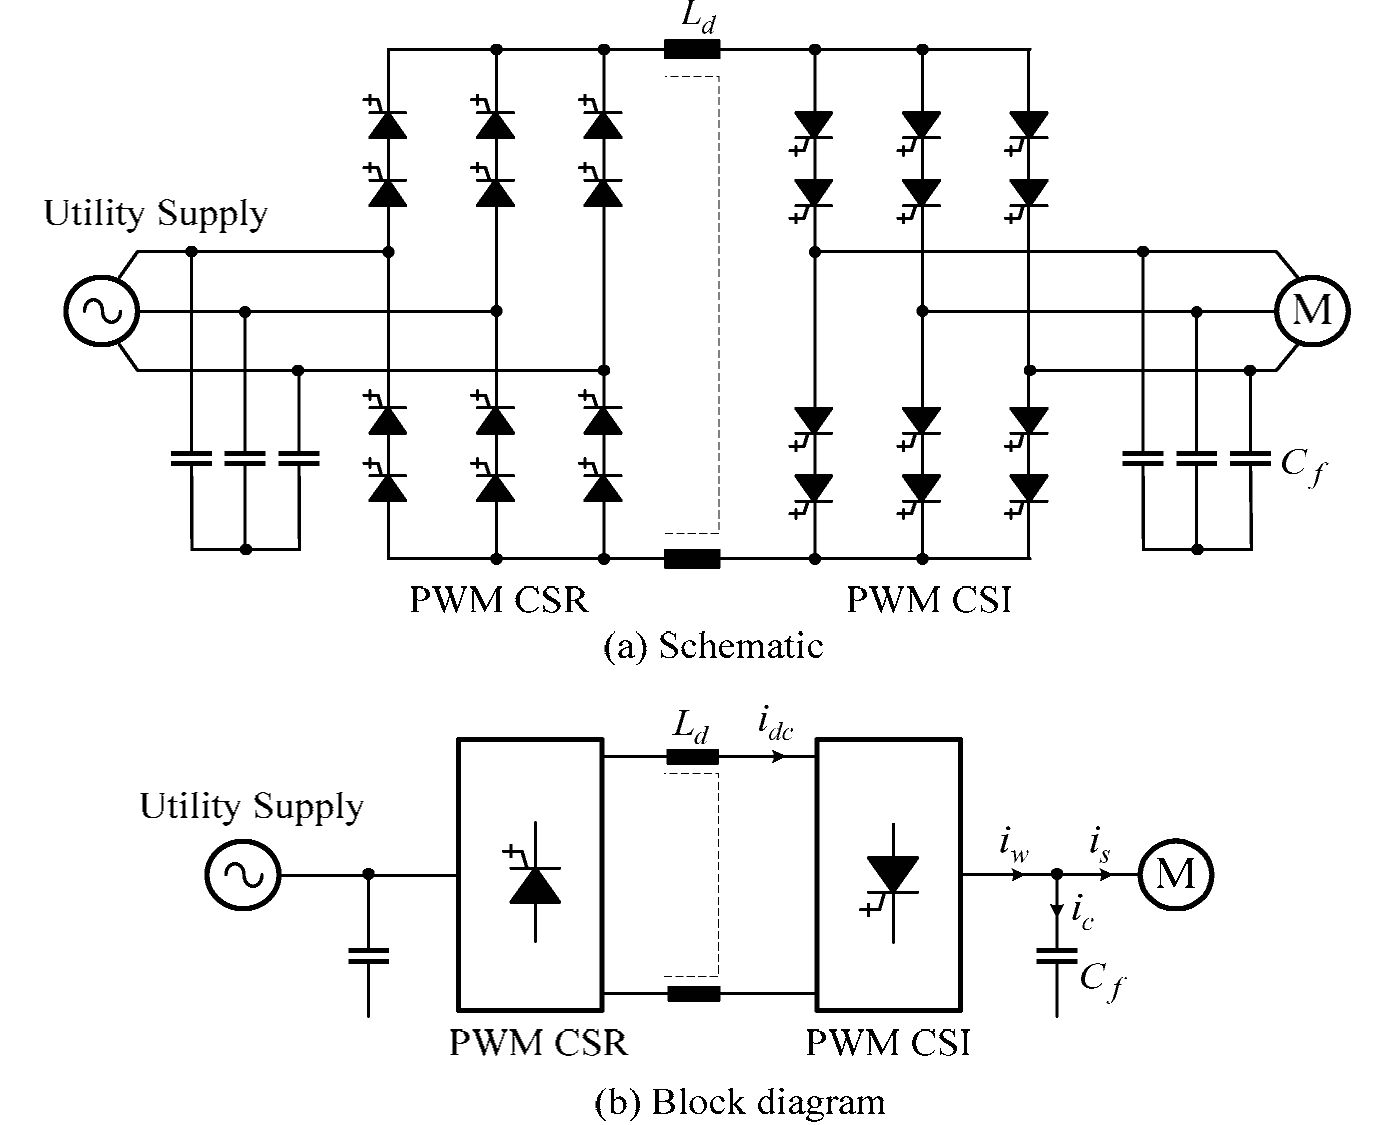
\includegraphics{graficos/img20.jpg}
\caption{Figure 14.7-1: A PWM current source converter-based drive.}
\end{figure}
\FloatBarrier

In VSI-fed MV drives, both inverter output voltage and frequency can be controlled by its PWM scheme. However, this is not the case for the CSI-fed drive shown in Fig. 14.7-1, where the inverter output frequency is controlled by its PWM scheme whereas the inverter output current $\vec{i}_w$ is adjusted by dc current $i_{dc}$ of the rectifier. In addition, the stator current $\vec{i}_s$ is not directly controlled by $\vec{i}_w$ due to the filter capacitor $C_f$. Therefore, additional measures are required to maintain field orientation in CSI drives.

\begin{figure}[h]
\centering
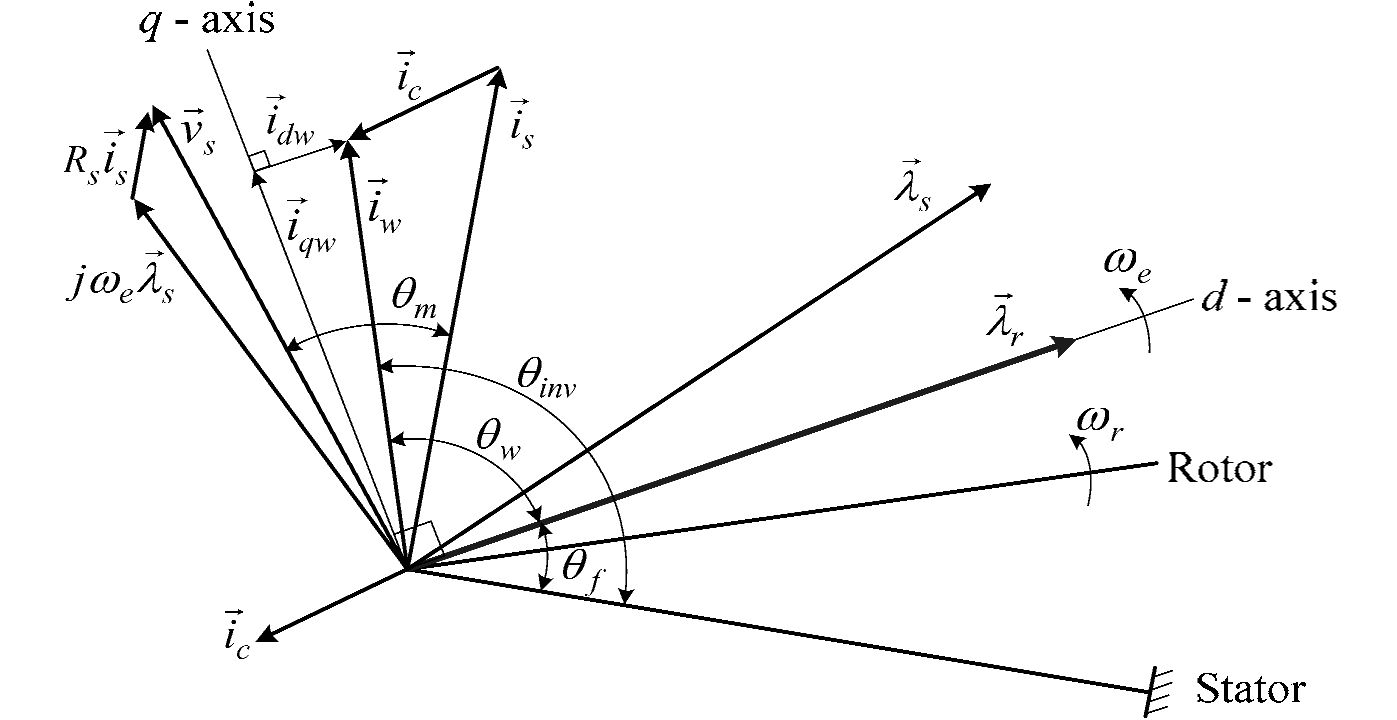
\includegraphics{graficos/img21.jpg}
\caption{Figure 14.7-2: Vector diagram for a CSI-fed drive with rotor flux orientation.}
\end{figure}
\FloatBarrier

Figure 14.7-2 shows the space vector diagram for the CSI drive with rotor flux oriented control. The $d$-axis of the synchronous reference frame is aligned with the rotor flux vector $\vec{\lambda}_r$. The stator flux vector $\vec{\lambda}_s$ leads the rotor flux $\vec{\lambda}_r$ by a small angle due to the leakage inductances. The stator voltage $\vec{v}_s$ is the sum of the speed voltage $j\omega \vec{\lambda}_s$ and the stator resistance voltage drop $R_s \vec{i}_s$. The stator current $\vec{i}_s$ lags $\vec{v}_s$ by $\theta_{m}$, which is the motor power factor angle. The capacitor current $\vec{i}_c$ leads $\vec{v}_s$ by $\pi/2$. The inverter PWM current $\vec{i}_w$ is a vector sum of $\vec{i}_s$ and $\vec{i}_c$, and its angle with respect to $\vec{\lambda}_r$ is $\theta_{w}$. The inverter firing angle is

\begin{equation}
\theta_{inv} = \theta_{w} + \theta_{f} \tag{14.7-1}
\end{equation}

where $\theta_{f}$ is the rotor flux angle for field orientation. When the drive operates in steady state, $\theta_{w}$ is constant since both $\vec{i}_w$ and $\vec{\lambda}_r$ are in the synchronous reference frame while $\theta_{f}$ and $\theta_{inv}$ vary periodically between zero and $2\pi$.

\begin{figure}[h]
\centering
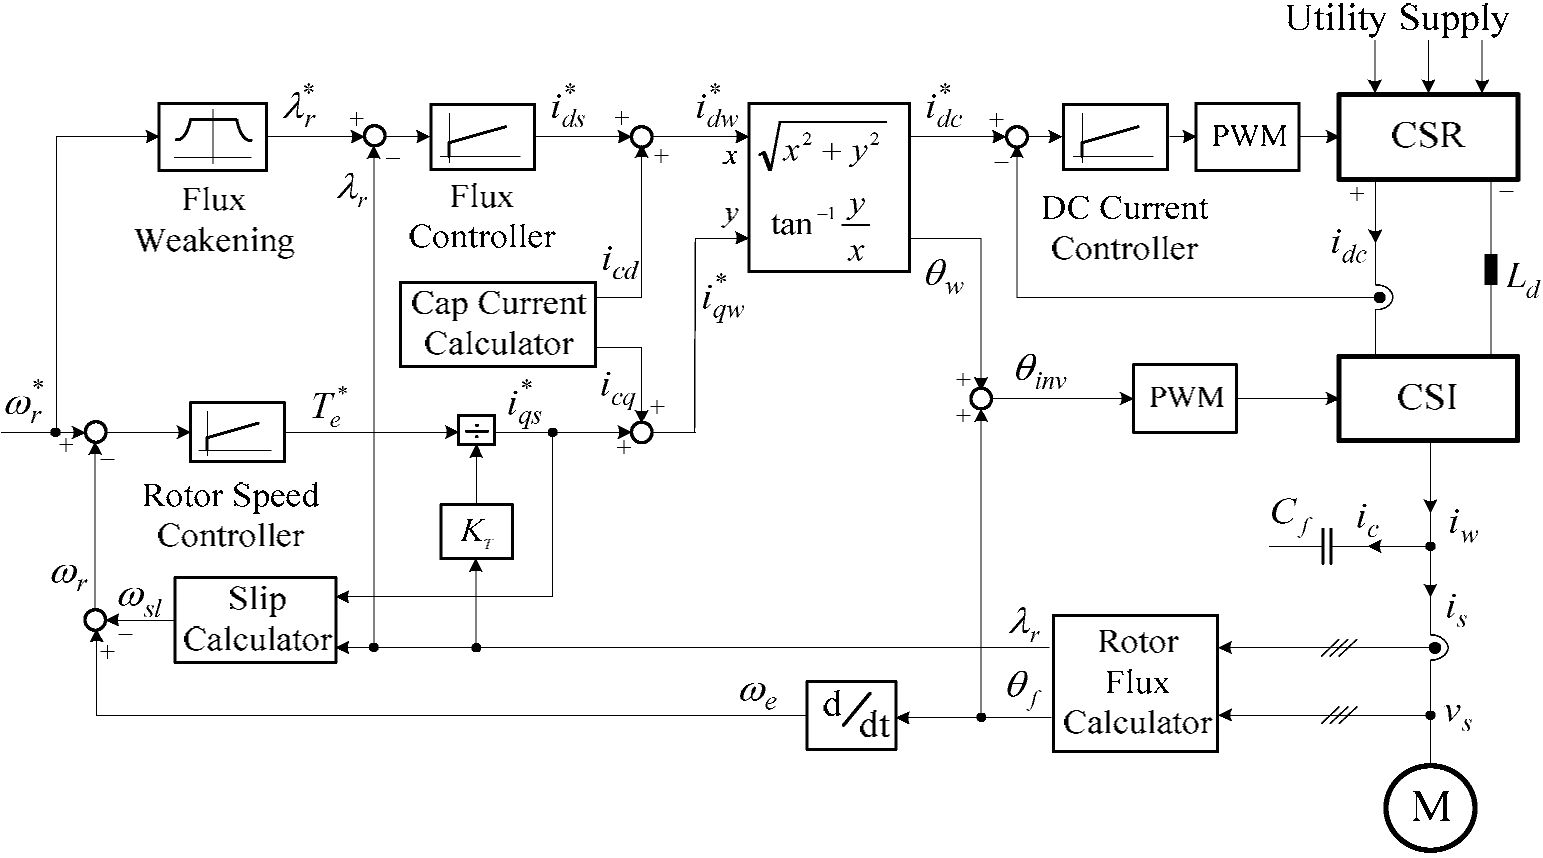
\includegraphics{graficos/img22.jpg}
\caption{Figure 14.7-3: Simplified block diagram for a CSI-fed drive using direct FOC scheme.}
\end{figure}
\FloatBarrier

Figure 14.7-3 shows a simplified block diagram for the CSI-fed drive with direct field-oriented control. The FOC scheme is implemented with three feedback control loops, one for the rotor speed $\omega_r$, one for the rotor flux $\lambda_r$, and another for the dc current $i_{dc}$. The rotor speed $\omega_r$ is obtained by $\omega_r = \omega_e - \omega_{sl}$ where $\omega_e = d\theta_f / dt$ and $\omega_{sl}$ can be calculated by (14.6-8).

The $q$-axis (torque-producing) stator current reference $i_{qs}^*$ and $d$-axis (flux-producing) current reference $i_{ds}^*$ are generated in the same manner as that shown in Fig. 14.5-1. The $dq$-axis inverter PWM current references can be expressed as

\begin{equation}
i_{dw}^* = i_{cd} + i_{ds}^* \tag{14.7-2}
\end{equation}

\begin{equation}
i_{qw}^* = i_{cq} + i_{qs}^* \tag{14.7-3}
\end{equation}

where $i_{cd}$ and $i_{cq}$ are the $dq$-axis capacitor currents, given by

\begin{equation}
i_{cd} = (p v_{ds} - \omega_e v_{qs}) C_f \tag{14.7-4}
\end{equation}

\begin{equation}
i_{cq} = (p v_{qs} + \omega_e v_{ds}) C_f \tag{14.7-5}
\end{equation}

The first term on the right-hand side of the equation represents capacitor transient current, and the second term is the steady-state current. To reduce the sensitivity and noise caused by the derivative terms $(p v_{ds}$ and $p v_{qs})$, the effect of the capacitor transient response on the drive dynamic performance may be neglected. Equation (14.7-3) can then be simplified to

\begin{equation}
i_{cd} = \omega_e v_{qs} C_f \tag{14.7-6}
\end{equation}

\begin{equation}
i_{cq} = \omega_e v_{ds} C_f \tag{14.7-7}
\end{equation}

for use in the Capacitor Current Calculator in Fig. 14.7-3.

Since the magnitude of $i_w$ is proportional to the dc current, the dc current reference can be found from

\begin{equation}
i_{dc}^* = \sqrt{(i_{dw}^*)^2 + (i_{qw}^*)^2} \tag{14.7-8}
\end{equation}

The inverter firing angle $\theta_{inv}$ is the sum of $\theta_f$ and $\theta_w$, where $\theta_f$ can be obtained from the Rotor Flux Calculator in Fig. 14.5-3 and $\theta_w$ can be determined by

\begin{equation}
\theta_w = \tan^{-1} (i_{qw}^* / i_{dw}^*) \tag{14.7-9}
\end{equation}

Various PWM schemes, such as SHE, TPWM, and SVM presented in Chapters 10 and 11, can be employed for the PWM blocks in Fig. 14.7-3.

\section{Direct Torque Control}
Direct torque control (DTC) is one of the advanced control schemes for ac drives [5-7]. It is characterized by simple control algorithm, easy digital implementation and robust operation [8, 9]. In this section, the principle of DTC scheme is introduced and simulation results are provided.

\subsection{Principle of Direct Torque Control}
The electromagnetic torque developed by an induction motor can be expressed in a number of ways, one of which is

\begin{equation}
T_e = \frac{3P}{2} \frac{L_m}{\sigma L_s L_r} \lambda_s \lambda_r \sin \theta_r \tag{14.8-1}
\end{equation}

where $\theta_r$ is the angle between the stator flux vector $\vec{\lambda_s}$ and rotor flux vector $\vec{\lambda_r}$, often known as torque angle. This equation indicates that $T_e$ can be directly controlled by $\theta_r$.

The main variable to be controlled in the DTC scheme is the stator flux vector $\vec{\lambda_s}$. Referring to the induction motor model of Fig. 14.3-2b, $\vec{\lambda_s}$ relates the stator voltage vector $\vec{v_s}$ by

\begin{equation}
p \vec{\lambda_s} = \vec{v_s} - R_s \vec{i_s} \tag{14.8-2}
\end{equation}

The equation shows that the derivative of $\vec{\lambda_s}$ reacts instantly to changes in $\vec{v_s}$. As discussed in Chapter 6, the stator voltage $\vec{v_s}$, which is the inverter output voltage, can be controlled by the reference vector $\vec{V_{ref}}$ in the space vector modulation. Since $\vec{V_{ref}}$ is synthesized by the stationary voltage vectors of the inverter, a proper selection of the stationary vectors can make the magnitude and angle of $\vec{\lambda_s}$ adjustable.

\begin{figure}[h]
\centering
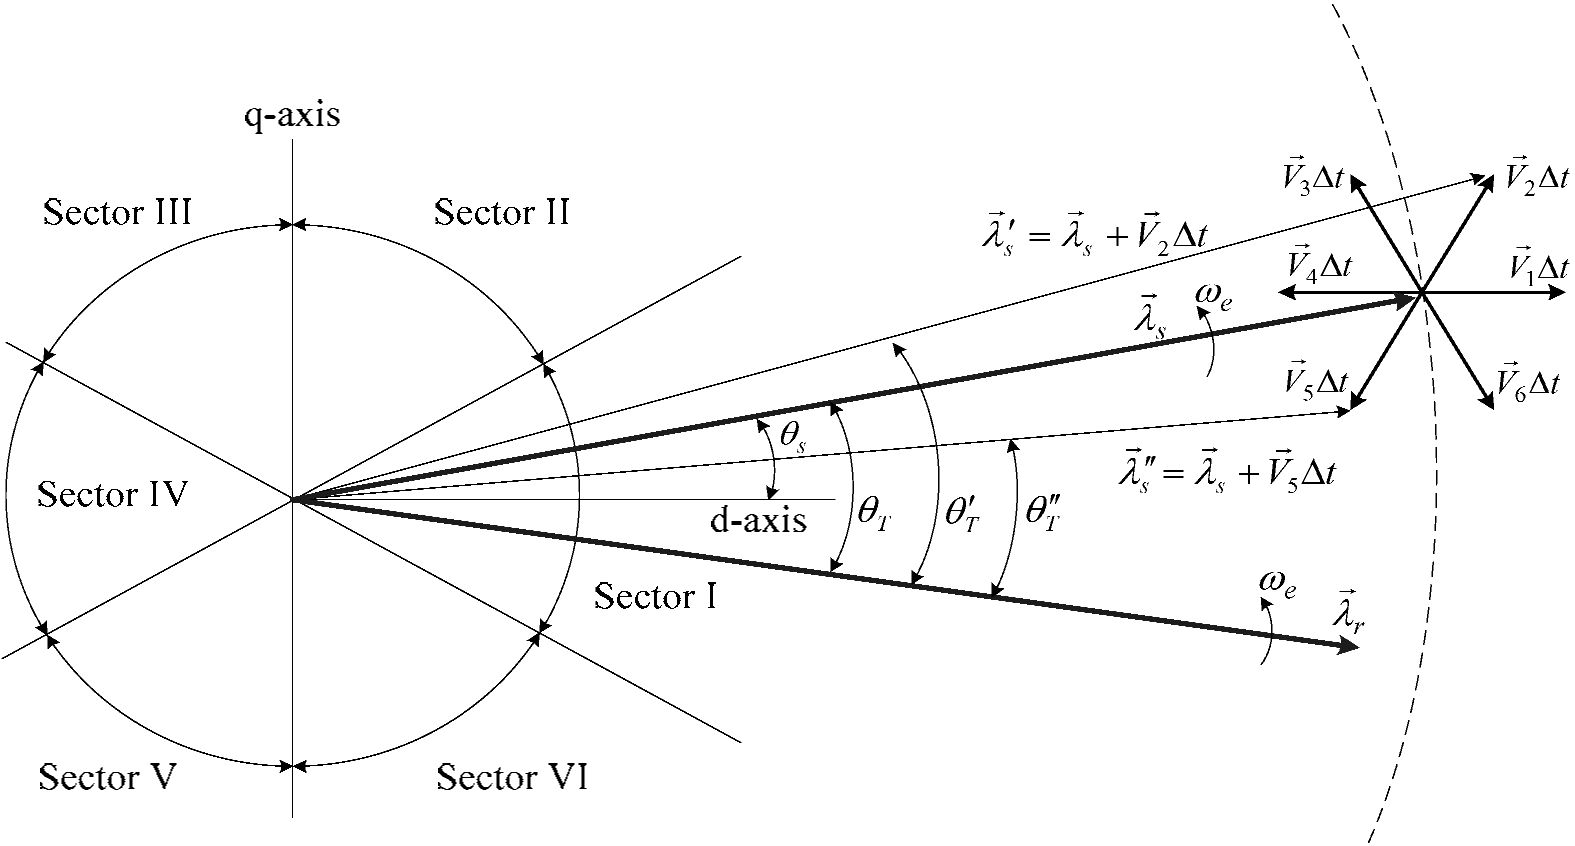
\includegraphics{graficos/img23.jpg}
\caption{Figure 14.8-1: Principle of direct torque control.}
\label{fig:14.8-1}
\end{figure}
\FloatBarrier

Figure 14.8-1 shows the principle of direct torque control for a two-level VSI-fed induction motor drive. The $dq$-axis plane for the stator flux $\vec{\lambda_s}$ is divided into six sectors I to VI. The stator flux $\vec{\lambda_s}$ in the figure falls into sector I, and its angle $\theta_s$ is referenced to the d-axis of the stationary reference frame. The rotor flux vector $\vec{\lambda_r}$ lags $\vec{\lambda_s}$ by $\theta_r$.

Let’s now examine the impact of the stationary voltage vectors $\vec{V_0}$ to $\vec{V_6}$ on $\vec{\lambda_s}$ and $\theta_r$. Assume that $\vec{\lambda_s}$ and $\theta_r$ in Fig. 14.8-1 are the initial stator flux vector and torque angle. When voltage vector $\vec{V_2}$ is selected, the stator flux vector will become $\vec{\lambda_s}' = \vec{\lambda_s} + \vec{V_2}\Delta t$ after a short time interval $\Delta t$, leading to an increase in flux magnitude ($\lambda_s' > \lambda_s$) and torque angle ($\theta_r' > \theta_r$). If voltage vector $\vec{V_5}$ is selected, $\vec{\lambda_s}$ will change to $\vec{\lambda_s}'' = \vec{\lambda_s} + \vec{V_5}\Delta t$, causing a decrease in flux magnitude ($\lambda_s'' < \lambda_s$) and torque angle ($\theta_r'' < \theta_r$). Similarly, the selection of $\vec{V_3}$ and $\vec{V_6}$ can make one variable increase and the other decrease. Therefore, $\lambda_s$ and $\theta_r$ can be controlled separately by proper selection of the inverter voltage vectors.

Note that the changes in $\vec{v_s}$ have much less impact on $\vec{\lambda_r}$ for a short time interval $\Delta t$ due to the large rotor time constant. Therefore, it is assumed in the above analysis that the rotor flux vector $\vec{\lambda_r}$ is kept constant during $\Delta t$.

\subsection{Switching Logic}

\begin{figure}[h]
\centering
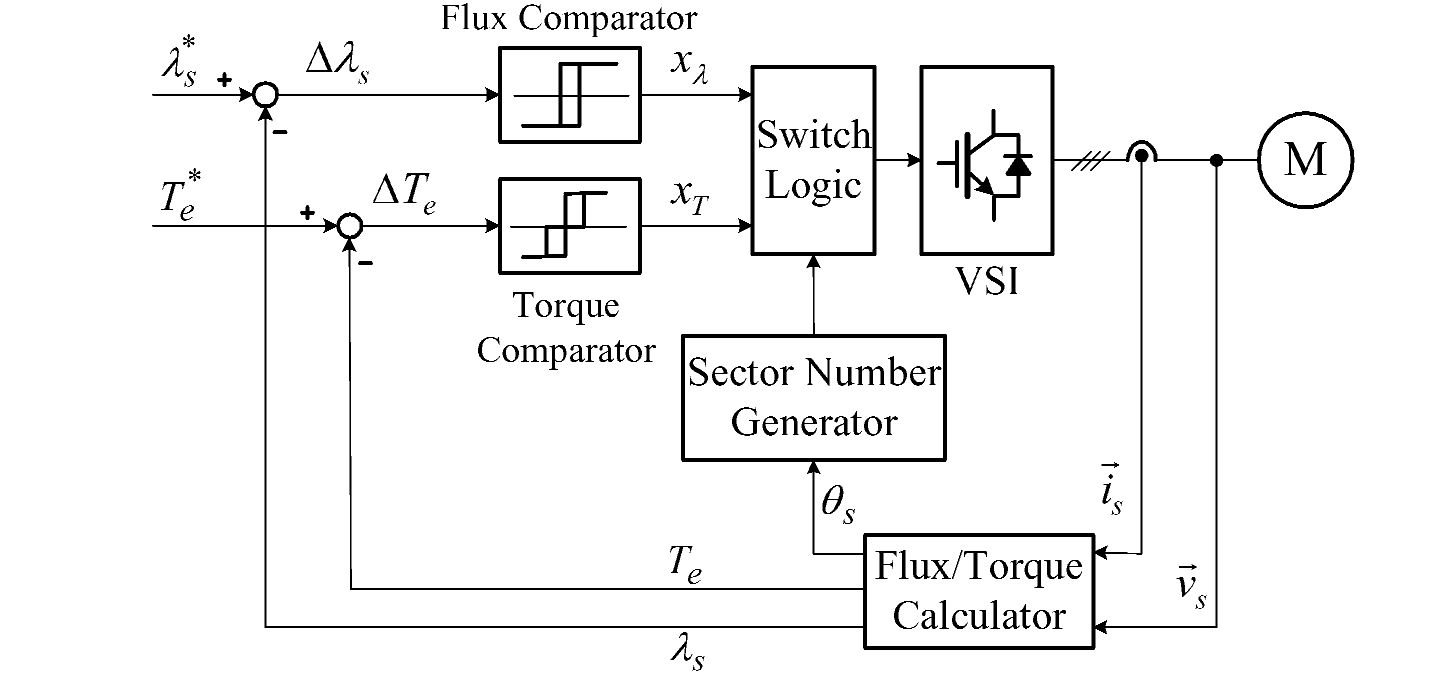
\includegraphics{graficos/img24.jpg}
\caption{Figure 14.8-2: Block diagram of direct torque control scheme.}
\label{fig:14.8-2}
\end{figure}
\FloatBarrier

Figure 14.8-2 shows a typical block diagram of a DTC-based induction motor drive, where the rotor speed feedback loop is not shown for simplicity. Similar to the FOC schemes, the stator flux and electromagnetic torque are controlled separately to achieve superior dynamic performance. The stator flux reference $\lambda_s^*$ is compared with the calculated stator flux $\lambda_s$, and the error $\Delta \lambda_s$ is sent to Flux Comparator. The torque reference $T_e^*$ is compared with the calculated torque $T_e$, and their difference $\Delta T_e$ is the input of Torque Comparator. The output of the flux and torque comparators ($\chi_\lambda$ and $\chi_T$) are sent to Switching Logic unit for proper selection of the voltage vectors (switching states) of the inverter.

\begin{figure}[h]
\centering
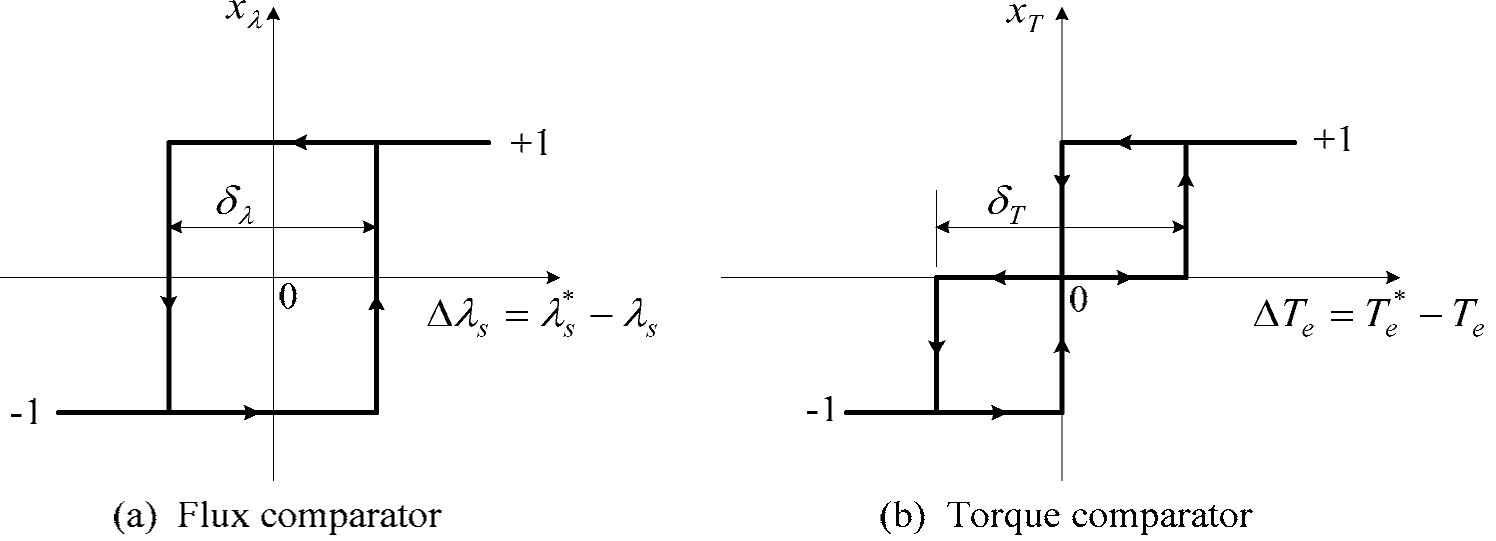
\includegraphics{graficos/img25.jpg}
\caption{Figure 14.8-3: Characteristics of hysteresis comparators.}
\label{fig:14.8-3}
\end{figure}
\FloatBarrier

Both flux and torque comparators are of a hysteresis (tolerance band) type, whose transfer characteristics are shown in Fig. 14.8-3. The flux comparator has two output levels ($\chi_\lambda = +1$ and $-1$) while the torque comparator has three output levels ($\chi_T = +1, 0$ and $-1$), where "+1" requests an increase in $\lambda_s$ or $\theta_r$, "-1" demands a decrease in $\lambda_s$ or $\theta_r$, and "0" signifies no changes. The tolerance band for the flux and torque comparators is $\delta_\lambda$ and $\delta_T$, respectively.

\begin{figure}[h]
\centering
\caption{Table 14.8-1: Switching Logic for $\vec{\lambda_s}^*$ Rotating in the Counterclockwise Direction.}
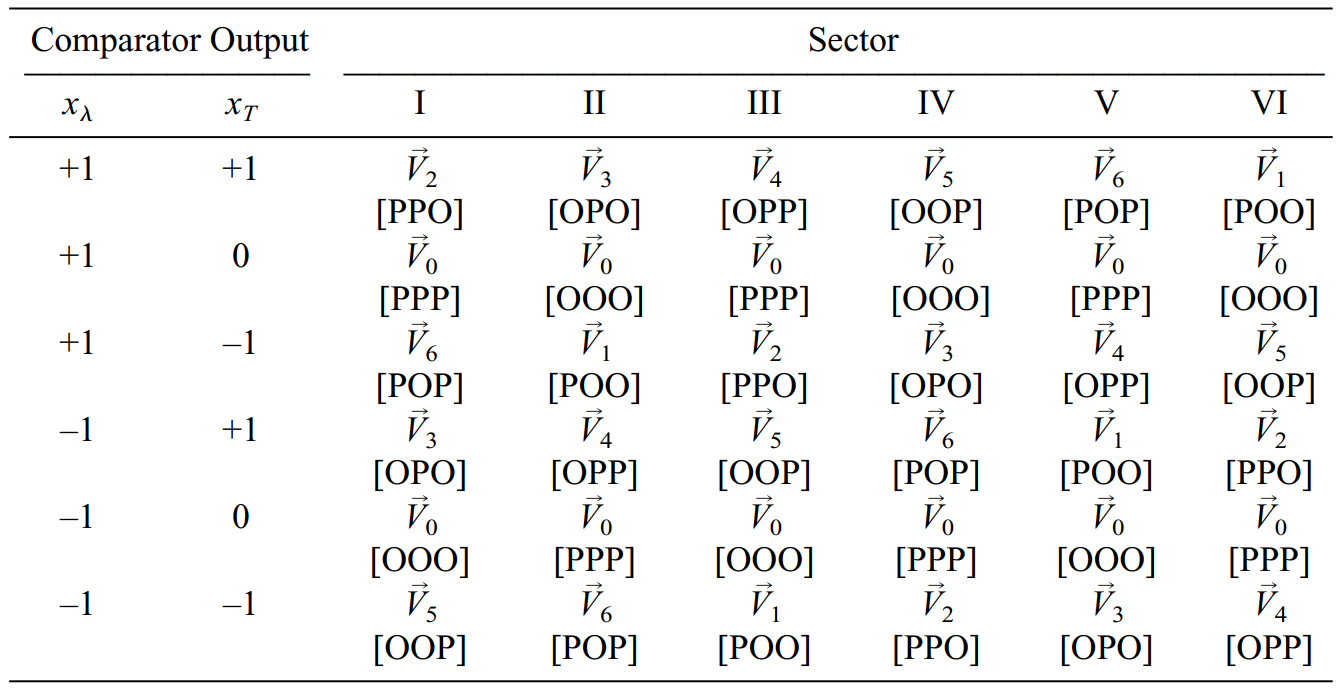
\includegraphics[scale=0.4]{graficos/tabla_14_8_1.png}
\label{tab:14.8-1}
\end{figure}
\FloatBarrier

Table 14.8-1 gives the switching logic for the stator flux reference $\vec{\lambda_s}^*$ rotating in the counterclockwise direction. The input variables are $\chi_\lambda$, $\chi_T$, and the sector number, and the output variables are the inverter voltage vectors. The output of the comparators decides which voltage vector should be selected. Assuming that $\vec{\lambda_s}^*$ is in sector I, the comparator output of $\chi_\lambda = \chi_T = +1$ signifies an increase in $\lambda_s$ and $T_e$. Voltage vector $\vec{V_2}$ can then be selected from the table. This selection will make both $\lambda_s$ and $\theta_r$ increase as shown in Fig. 14.8-1.

When the output of the torque comparator $\chi_T$ is zero (no need to adjust $T_e$), zero vector $\vec{V_0}$ can be selected. The alternative use of the switching states [OOO] and [PPP] for $\vec{V_0}$ in the switching table can help to reduce the device switching frequency. For instance, when $\chi_T$ changes between ‘+1’ and ‘0’ or between ‘0’ and ‘-1’, the zero states in the table ensures that only two switches are involved during the transition, one being turned on and the other being turned off.

\begin{figure}[h]
\centering
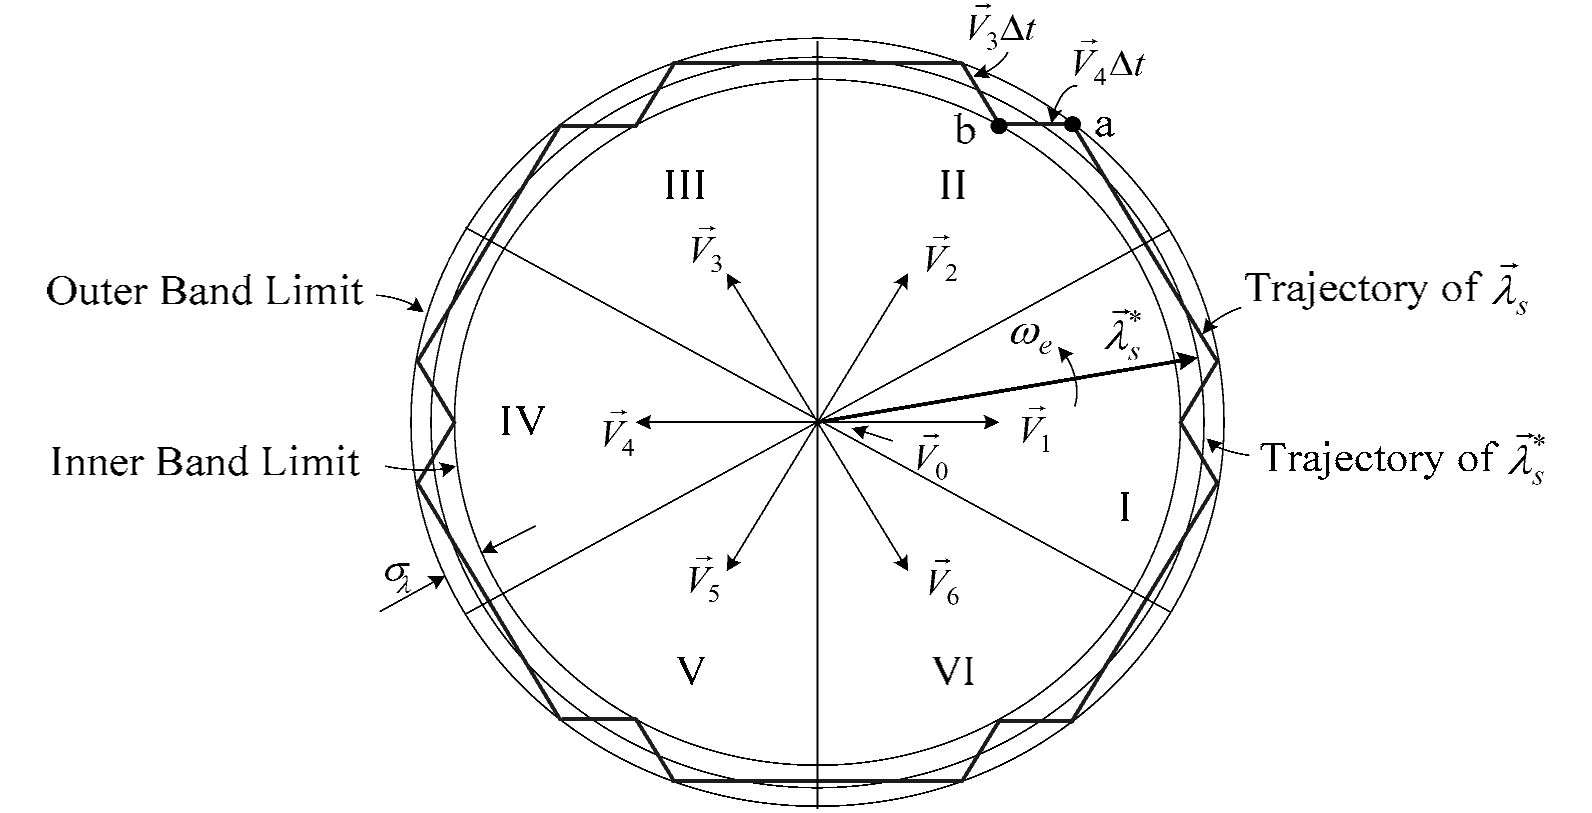
\includegraphics{graficos/img26.jpg}
\caption{Figure 14.8-4: Trajectories of the stator flux $\vec{\lambda_s}$ and its reference $\vec{\lambda_s}^*$ with $\chi_T = 1$.}
\label{fig:14.8-4}
\end{figure}
\FloatBarrier

The operation of the direct torque control can be further explained by the stator flux trajectory diagram of Fig. 14.8-4. Assume that the reference vector $\vec{\lambda_s}^*$ rotates in the counterclockwise direction during rotor speed acceleration and the output of the torque comparator is $\chi_T = +1$. When $\lambda_s$ reaches the outer band limit at point $a$ in sector II, the output of the flux comparator $\chi_\lambda$ becomes ‘-1’, and vector $\vec{V_4}$ is selected from the switching table, which will cause a decrease in $\lambda_s$. When $\lambda_s$ hits the inner band limit at point $b$, $\chi_\lambda$ becomes +1, and vector $\vec{V_3}$ is selected, making an increase in $\lambda_s$. The trajectory of $\vec{\lambda_s}$ in the figure is not very smooth due to the wide width of the tolerance band $\delta_\lambda$, which translates into a high stator flux ripple and low switching frequency. The quality of the stator flux waveform can be improved by reducing $\delta_\lambda$, but it is achieved at the expense of an increase in the switching frequency.

\begin{figure}[h]
\centering
\caption{Table 14.8-2: Switching Logic for the Stator Flux Rotating in the Clockwise Direction}
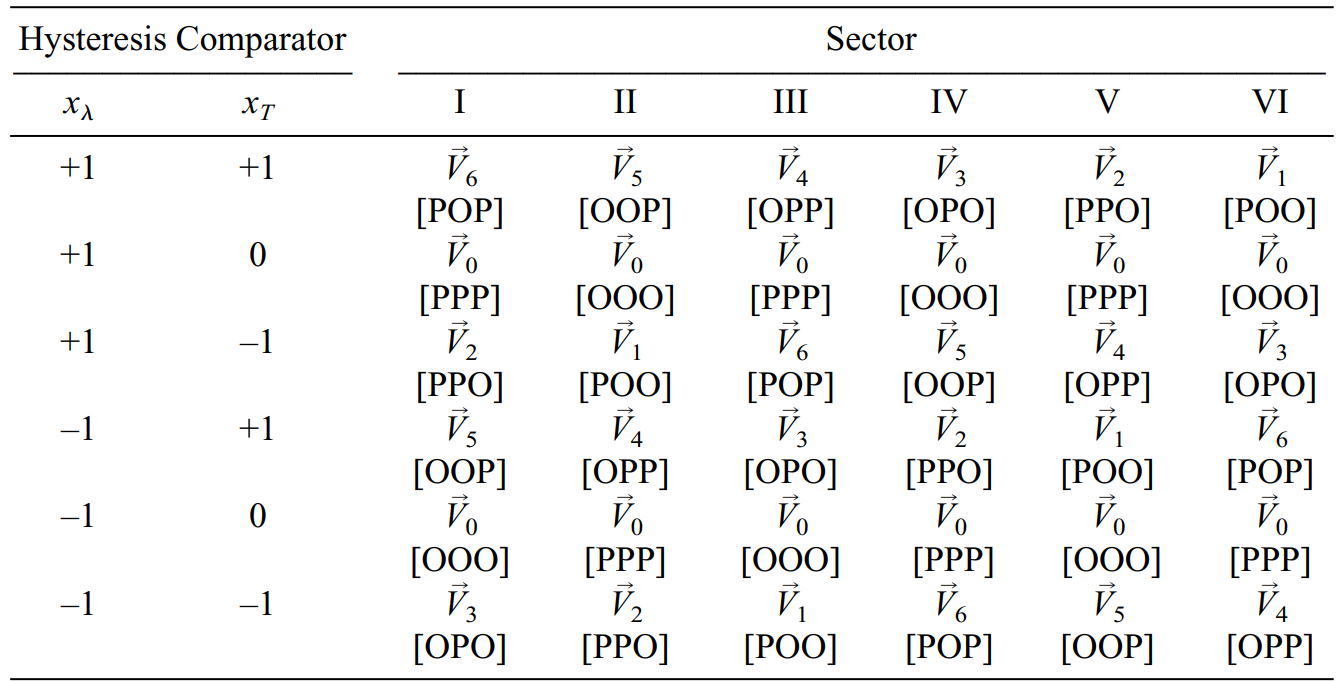
\includegraphics[scale=0.4]{graficos/tabla_14_8_2.png}
\label{tab:14.8-2}
\end{figure}
\FloatBarrier

The switching logic given in Table 14.8-1 is only valid for the motor rotating in the counterclockwise direction. When the motor operates in the clockwise direction, the switching logic in Table 14.8-2 can be used.

\subsection{Stator Flux and Torque Calculation}

The stator flux vector $\vec{\lambda_s}$ in the stationary frame can be expressed as
\begin{equation}
    \vec{\lambda_s} = \lambda_{ds} + j\lambda_{qs} = \int (v_{ds} - R_s i_{ds}) \, dt + j \int (v_{qs} - R_s i_{qs}) \, dt \tag{14.8-3}
\end{equation}

from which its magnitude and angle are
\begin{equation}
    \lambda_s = \sqrt{\lambda_{ds}^2 + \lambda_{qs}^2} \tag{14.8-4}
\end{equation}
\begin{equation}
    \theta_s = \tan^{-1} \left( \frac{\lambda_{qs}}{\lambda_{ds}} \right) \tag{14.8-5}
\end{equation}
where $v_{ds}$, $v_{qs}$, $i_{ds}$, and $i_{qs}$ are the measured stator voltages and currents. The developed electromagnetic torque can be calculated by
\begin{equation}
    T_e = \frac{3P}{2} \left( i_{qs} \lambda_{ds} - i_{ds} \lambda_{qs} \right) \tag{14.8-6}
\end{equation}

The above equations illustrate that the stator flux and developed torque can be obtained by using measured stator voltages and currents. The only motor parameter required in the calculations is the stator resistance $R_s$. This is in contrast to the direct rotor flux FOC schemes, where almost all the motor parameters are needed.

\subsection{DTC Drive Simulation}

\begin{figure}[h]
\centering
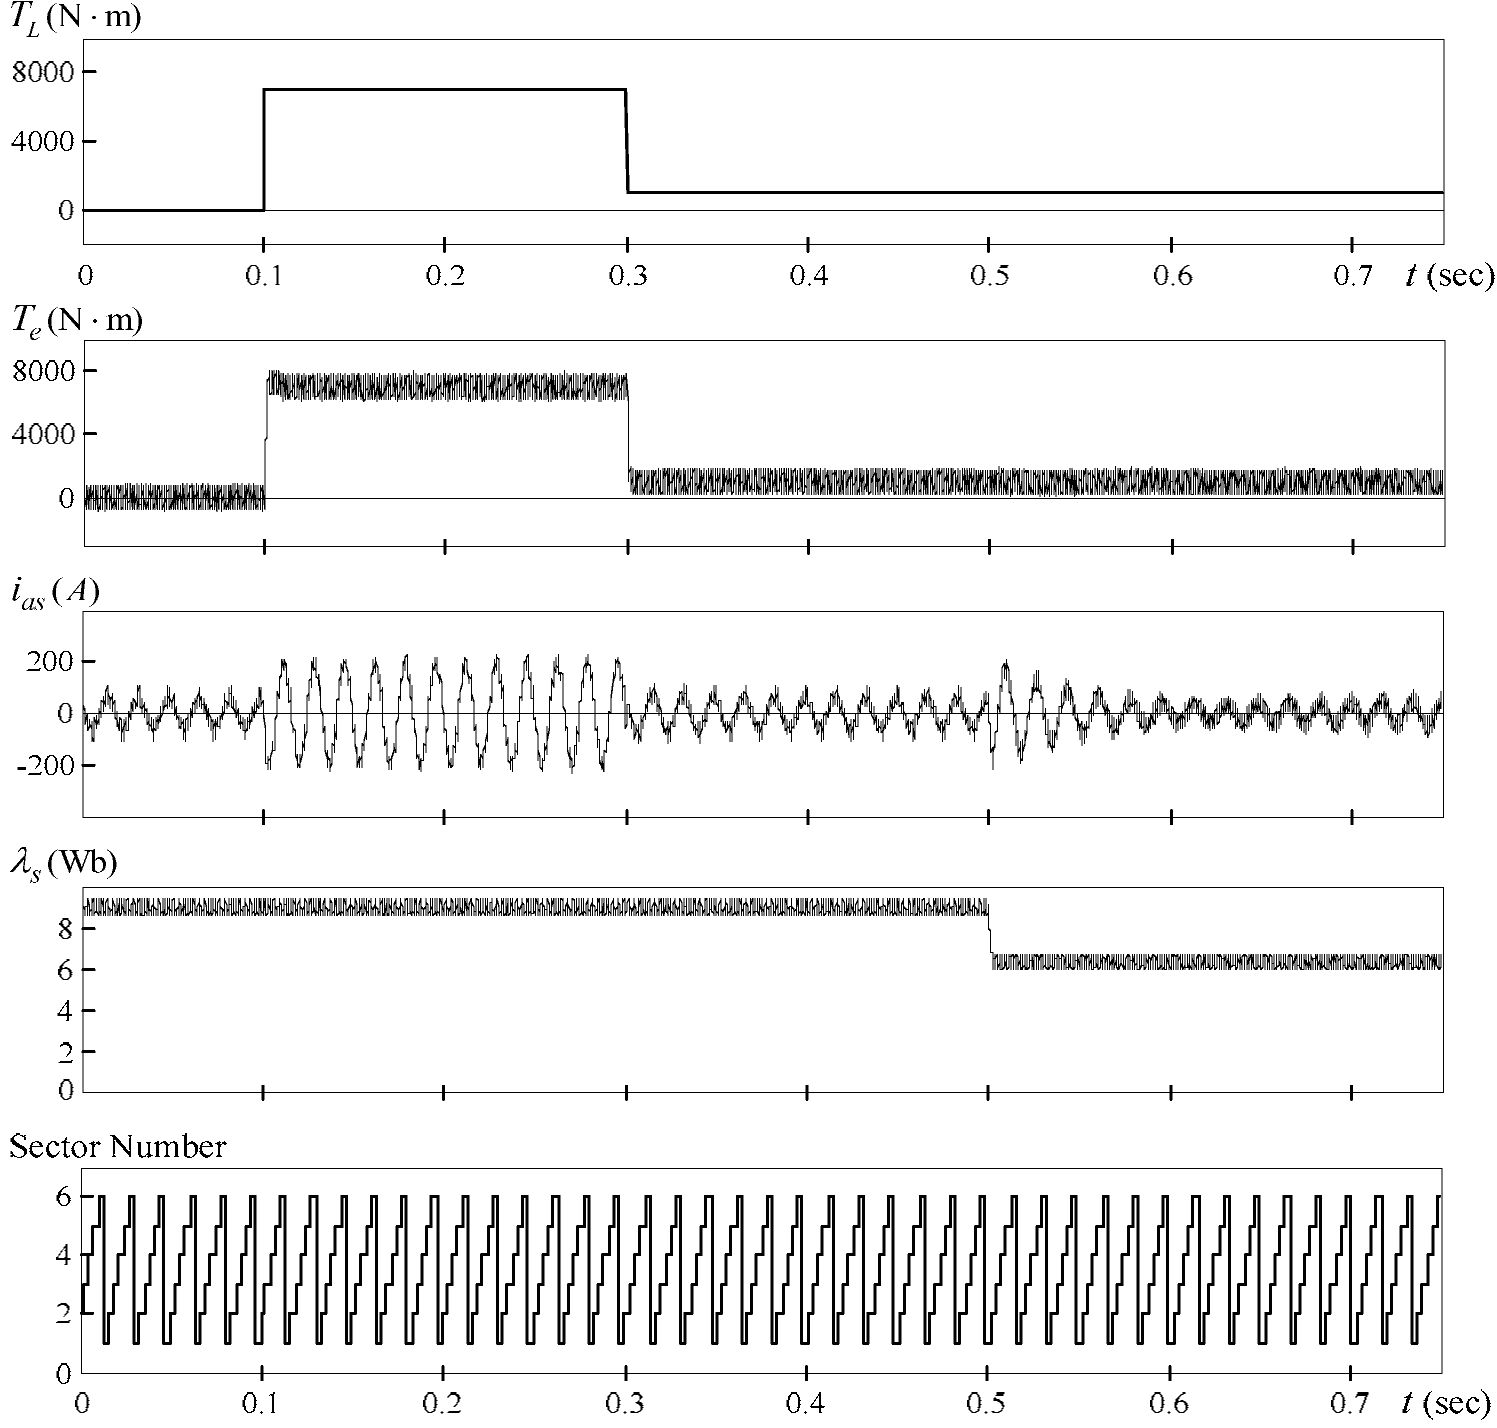
\includegraphics{graficos/img27.jpg}
\caption{Simulated waveforms for a DTC drive operating at the rated rotor speed.}
\label{fig:14.8-5}
\end{figure}
\FloatBarrier

Figure 14.8-5 shows the simulated waveforms for an induction motor drive using the DTC scheme given in Fig. 14.8-2. The rotor speed feedback loop, based on which the torque reference $T_e^*$ is generated, is not shown for simplicity. The motor parameters used in the simulation are given in Table 14.5-1.

The tolerance bands $\delta_T$ and $\delta_\lambda$ for the torque and flux comparators are adjusted such that average switching frequency $f_{sw}$ of the switching devices is around 800 Hz. The stator flux reference $\lambda_s^*$ is set to its rated value of 9.0 Wb.

The motor operates at the rated speed of $n_r = 1189$ rpm under no-load conditions. Assuming that the load torque $T_L$ is suddenly increased to its rated value of 7490 N·m at $t = 0.1$ s and then decreased to 1000 N·m at $t = 0.3$ s, the generated torque $T_e$ responds quickly. The torque ripple is set by the torque tolerance band $\delta_T$. The stator current $i_{as}$ varies with $T_e$ accordingly.

Since the stator flux $\lambda_s$ and the motor torque $T_e$ are controlled independently, $\lambda_s$ is kept constant during the sudden load torque changes. To demonstrate the effectiveness of the stator flux control, its reference $\lambda_s^*$ has a step reduction from its rated value of 9.0 Wb to 6.3 Wb at $t = 0.5$ s. The stator flux $\lambda_s$ responds quickly while the stator current $i_{as}$ is adjusted accordingly to keep $T_e$ constant. The sector number obtained from the sector number generator in Fig. 14.8-2 is also shown in the figure.

\begin{figure}[h]
\centering
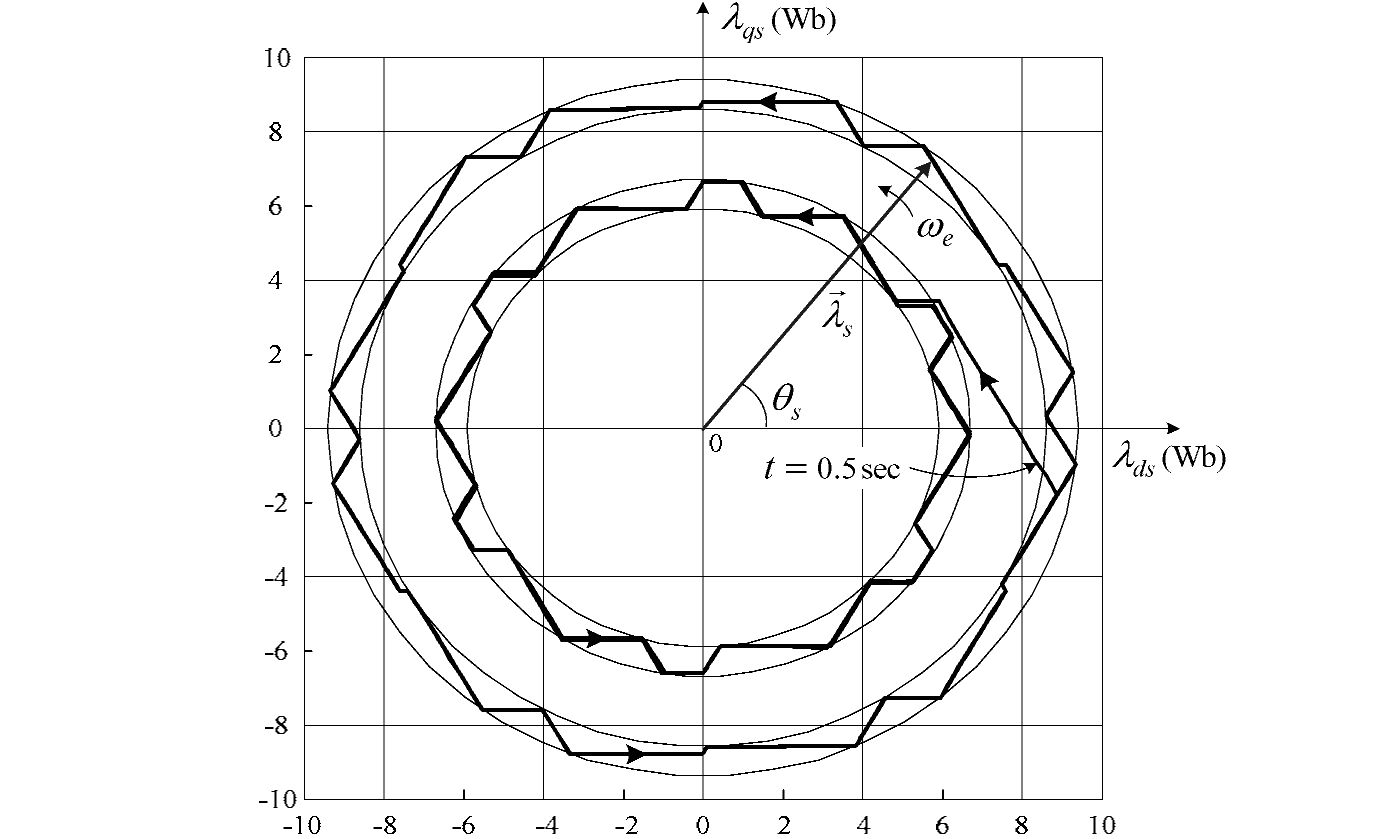
\includegraphics{graficos/img28.jpg}
\caption{Trajectories of the stator flux $\lambda_s$ in Fig. 14.8-5 for $0.35 \leq t \leq 0.75$ s.}
\label{fig:14.8-6}
\end{figure}
\FloatBarrier

Figure 14.8-6 shows the trajectories of the stator flux $\lambda_s$ in Fig. 14.8-5 for $0.35 \leq t \leq 0.75$ s. The outer and inner trajectories correspond to the steady-state operation before and after the stator flux reduction at $t = 0.5$ s.

\subsection{Comparison Between DTC and FOC Schemes}

\begin{table}[h]
    \centering
    \caption{Table 14.8-3 Comparison Between DTC and FOC Schemes}
    \begin{tabular}{l l l}
        \hline
        \textbf{Comparison} & \textbf{DTC} & \textbf{FOC} \\
        \hline
        Field orientation (Reference & Not required & Required \\
            frame transformation) & & \\
        Control scheme & Simple & Complex \\
        Stator current control & No & Yes \\
        Motor parameters required & $R_s$ & $R_s$, $L_{ls}$, $L_{lr}$, $L_m$, and $R_r$ \\
        Sensitivity to motor parameter & Not very sensitive & Sensitive \\
        variations & & \\
        PWM scheme & Hysteresis band & Carrier-based, SVM, or \\
        & & hysteresis band \\
        Switching behavior & Variable & Defined (for carrier- \\
        & & based and SVM) \\
        \hline
    \end{tabular}
    
    \label{table:14.8-3}
\end{table}
\FloatBarrier

Based on the analysis given in the preceding sections, the features and drawbacks for the DTC and rotor flux FOC schemes are summarized in Table 14.8-3.

\clearpage
\section{SUMMARY}

The field-oriented control (FOC) and direct torque control (DTC) schemes for high-performance MV drives are presented in this chapter. There exist a variety of field-oriented control schemes with many different variations and approaches. To make the subject matter easy to understand, this chapter focuses on the rotor flux oriented control schemes. The other reason for selecting such a scheme for detailed discussion lies in its simplicity and wide acceptance in the drive industry. The control algorithms for the direct and indirect rotor flux orientation are elaborated. In addition, the FOC for CSI-fed MV drives is introduced. The operating principle of the DTC scheme is discussed in detail, based on which a comparison between the two advanced schemes is provided.

The implementation of the FOC and DTC schemes requires accurate information on motor parameters. However, the motor parameters may vary with the operating conditions, such as rotor temperature rise and magnetic core saturation. The issues concerning the parameter sensitivity and on-line motor parameter tuning are out of the scope of this book, and therefore they are not addressed in this chapter.

\section*{REFERENCES}
\begin{enumerate}
    \item P. C. Krause, O. Wasynczuk, and S. D. Sudhoff, \textit{Analysis of Electric Machines and Drive Systems}, 2nd edition, Wiley-IEEE Press, New York, 2002.
    \item I. Boldear and S. A. Nasar, \textit{Electric Drives}, CRC Press, Boca Raton, FL, 1999.
    \item D. W. Novotny and T. A. Lipo, \textit{Vector Control and Dynamics of AC Drives}, Clarendon Press, New York, 1996.
    \item P. Vas, \textit{Sensorless Vector and Direct Torque Control}, Oxford University Press, New York, 1998.
    \item J. N. Nash, ``Direct Torque Control, Induction Motor Vector Control Without an Encoder,'' \textit{IEEE Transaction on Industry Applications}, Vol. 33, No. 2, pp. 333--341, 1997.
    \item P. Pohjolainen and C. Stulz, ``Method and Apparatus for Direct Torque Control of a Three-Phase Machine,'' US Patent 5,734,249, 9 pages, March 1998.
    \item S. Heikkila, ``Direct Torque Control Inverter Arrangement,'' US Patent 6,094,364, 13 pages, July 2000.
    \item D. Casadei, F. Profumo, and A. Tani, ``FOC and DTC: Two Viable Schemes for Induction Motors Torque Control,'' \textit{IEEE Transactions on Power Electronics}, Vol. 17, No. 5, pp. 779--787, 2002.
    \item D. Telford, M. W. Dunnigan, and B. W. Williams, ``A Comparison of Vector Control and Direct Torque Control of an Induction Machine,'' \textit{IEEE Power Electronics Specialists Conference (PESC)}, Vol. 1, pp. 421--426, 2000.
\end{enumerate}

\clearpage
\section*{Abbreviations}

\begin{flushleft}
\begin{tabular}{ll}
ABB & Asea-Brown-Boveri \\
APOD & Alternative phase opposite disposition \\
CHB & Cascade H-bridge \\
CSI & Current source inverter \\
CSR & Current source rectifier \\
DF & Distortion factor \\
DPF & Displacement power factor \\
DTC & Direct torque control \\
ETO & Emitter turn-off thyristor \\
FC & Flux controller \\
FOC & Field oriented control \\
GCT & Gate commutated thyristor (also known as integrated gate commutated thyristor) \\
GTO & Gate turn-off thyristor \\
HPF & High pass filter \\
IEEE & Institute of Electrical and Electronics Engineers \\
IEGT & Injection enhanced gate transistor \\
IGBT & Insulated gate bipolar transistor \\
IPD & In-phase disposition \\
LCI & Load commutated inverter \\
LPF & Low pass filter \\
MCT & MOS controlled thyristor \\
MOSFET & Metal-oxide semiconductor field-effect transistor \\
MV & Medium voltage (2.3 KV to 13.8 KV) \\
NPC & Neutral point clamped \\
PCBB & Power converter building block \\
PF & Power factor (DF x DPF) \\
PI & Proportional and integral \\
PLL & Phase-locked loop \\
POD & Phase opposite disposition \\
PWM & Pulse width modulation \\
pu & Per unit \\
rms & Root mean square \\
rpm & Revolutions per minute \\
SCR & Silicon controlled rectifier (thyristor) \\
SHE & Selective harmonic elimination \\
SIT & Static induction thyristor \\
SM & Synchronous motor \\
SPWM & Sinusoidal pulse width modulation \\
SVM & Space-vector modulation \\
THD & Total harmonic distortion \\
TPWM & Trapezoidal pulse width modulation \\
VSI & Voltage source inverter \\
\end{tabular}
\end{flushleft}

\begin{flushright}
\textit{High-Power Converters and ac Drives. By Bin Wu}
\newline
© 2006 The Institute of Electrical and Electronics Engineers, Inc.
\end{flushright}

\end{document}
